\documentclass[9pt,a4paper,twocolumn,lineno]{article}
\usepackage[margin=.8in]{geometry}
\usepackage{graphicx}
\usepackage{amsmath}
\usepackage{amssymb}
\usepackage{titlesec}
\usepackage[numbers]{natbib}
\usepackage{sidecap, caption}
\usepackage{subcaption}
\usepackage[figuresleft]{rotating}
\usepackage{fixme}
\usepackage{tikz}
\usetikzlibrary{arrows,calc,matrix, arrows.meta,automata}
\tikzset{
%Define standard arrow tip
>=stealth',
%Define style for different line styles
help lines/.style={dashed, thick},
axis/.style={<->},
important line/.style={thick},
connection/.style={thick, dotted},
}
\usepackage{bm}
\renewcommand{\sfdefault}{mdugm}
\graphicspath{{../plots/}}

\newcommand{\at}{\makeatletter @\makeatother}
\titlespacing*{\section}
{0pt}{2ex}{0ex}
\titlespacing*{\subsection}
{0pt}{2ex}{0ex}
\titlespacing*{\subsubsection}
{0pt}{2ex}{0ex}
\graphicspath{{../plots/}}
\font\myfont=cmr12 at 16pt

\title{The Wisdom and Persuadability of Threads}
\author{(blinded)}
%\author{Robin Engelhardt$^1$, Vincent F. Hendricks$^1$ and Jacob Stærk-Østergaard$^1$}\\
%\textit{\small $^1$ Center for Information and Bubble Studies, Department of Communication,} \\
%\textit{\small University of Copenhagen, Karen Blixens Plads 8, DK-2300 Copenhagen S.}
%}
\date{}



\begin{document}

\twocolumn[
  \begin{@twocolumnfalse}
    \maketitle
    \begin{abstract}
\noindent
%Social decision-making is increasingly relying on digitized aggregates of people’s opinions and judgments. These aggregates are frequently maintained as threads, i.e. as sequences of posts on a website. While it has been shown that knowledge of thread aggregates can distort decision-making, it is unknown how seeing preceding posts in a thread may alter individual judgment and collective accuracy. We investigate experimentally the accuracy of threads in which people make magnitude estimations of varying difficulty while seeing a varying number of previous estimates. We find a significant increase in collective accuracy in difficult threads when the social information is pristine and  high levels social information in pristine threads, while collective accuracy declines quickly in manipulated threads. Using gaussian mixture models we assign a persuadability score to each participant, and show that persuadability generally increases with task difficulty and with the amount of social information. In the case of strong manipulation, we may see a split between a minority of persuadables and a majority of skeptics.
Online discussion threads are important means for individual decision-making and for aggregating collective judgments, e.g. the 'wisdom of crowds’. Empirical investigations of the wisdom of crowds are currently ambivalent about the role played by social information. While some findings suggest that social information undermines crowd accuracy due to correlated judgment errors, others show that accuracy improves. We investigate experimentally the accuracy of threads in which participants make magnitude estimates of varying difficulty while seeing a varying number of previous estimates. We demonstrate that, for difficult tasks, seeing preceding estimates aids the wisdom of crowds. If, however, participants only see extreme estimates, wisdom quickly turns into folly. Using a Gaussian Mixture Model, we assign a persuadability score to each participant and show that persuadability increases with task difficulty and with the amount of social information provided. In the filtered threads, we also see an increasing gap between highly persuadable participants and skeptics.
\\
\end{abstract}
  \end{@twocolumnfalse}
]


%
%\thispagestyle{firststyle}
%\ifthenelse{\boolean{shortarticle}}{\ifthenelse{\boolean{singlecolumn}}{\abscontentformatted}{\abscontent}}{}

Social information in the form of opinions and judgments by other people is sampled sequentially. We read the news, hear rumors, listen to debates on TV, and scroll through comments on social media platforms and blogs. These activities inform us and influence our decisions, but researchers still debate under what conditions these types of social information improve decisions-making \cite{woolley2010evidence, gurccay2015power, becker2017network, jayles2017social}, lead us astray \cite{caplan2011myth, lorenz2011social, minson2012cost, king2011true, le2018endogenous}, or simply add to our confusion \cite{salganik2006experimental, salganik2009web}.

Collective estimates of a diverse group of people can outperform the majority of its members because any random confusion at the individual level is likely to average out and let the most accurate estimate prevail \cite{galton1907vox, muth1961rational, surowiecki2005wisdom, hong2008some}. Then again, confusion is not always randomly scattered around the truth. Systematic biases in individual perceptions may create measurable disruptions in the wisdom of crowds \cite{izard2008calibrating, nash2014curious, kao2018counteracting}. Social information may add to those biases and create cascades, echo chambers, bandwagoning and herding behavior \cite{anderson1997information, bikhchandani1992theory, bakshy2015exposure, banerjee1992simple}. Partially sampled social information may lead to rich-get-richer dynamics \cite{barabasi1999emergence} and to belief misattributions, which uphold harmful social practices despite being rejected by a majority of people \cite{katz1931students, darley1968bystander, ross1977false, noelle1974spiral, lee2019homophily}. Social information may also have been intentionally filtered or manipulated in various ways, for instance through group pressure \cite{asch1951effects}, algorithmic filtering \cite{pariser2011filter}, false cues \cite{salganik2006experimental, muchnik2013social, hanson1996hits}, or simply by plain misinformation \cite{hendricks2018reality}, often with highly detrimental consequences for our economy and our health.

Observational data of decision-making processes is acutely sensitive to the social context in which people find themselves. Thus, researchers find it difficult to separate observational data into its social and individual components. How may we know how much weight an individual puts on her own ‘independent’ estimate relative to the weight put on the estimates by others? Randomized experimental studies have attempted to solve this problem by first letting participants make a magnitude estimate of an object without social information (\textit{ex ante}), and subsequently ask them to revise their estimate after having received information about other people’s estimates of that very object (\textit{ex post}) \cite{becker2017network, jayles2017social, lorenz2011social, sniezek1995cueing, mavrodiev2013quantifying}. This setup %double elicitation paradigm
presumes that people change their mind because of the social information they receive. Other studies, however, have shown that people routinely change their mind all by themselves, and that it may be more correct to assume an `inner crowd' in the sense that people sample randomly from a probability distribution in their own mind \cite{vul2008measuring, herzog2009wisdom, herzog2014harnessing}. Such a psychological mechanism - and perhaps others such as hedging strategies due to anticipated regrets \cite{bell1982regret}, and/or disappointments \cite{loomes1986disappointment} - make it difficult to differentiate between `inner' samples and `outer' influences. It is therefore desirable to develop an alternative framework that is able infer the extend of individual bias and social influence from a single estimation task.

We propose to use a probabilistic Gaussian Mixture Model (GMM) as it has properties that are highly valuable in crowd aggregation research. First, a GMM associates a measure to each data point, describing the influence of social information on that particular participant without any prior knowledge about that participant. Second, a GMM is comprised of several Gaussians which fit well to the right-skewed and heavy-tailed distributions emerging from free response elicitations. Finally, as a statistical model, a GMM provides confidence bounds to the estimates, which further adds a measure of model uncertainty.


\begin{figure*}[h]
\centering
	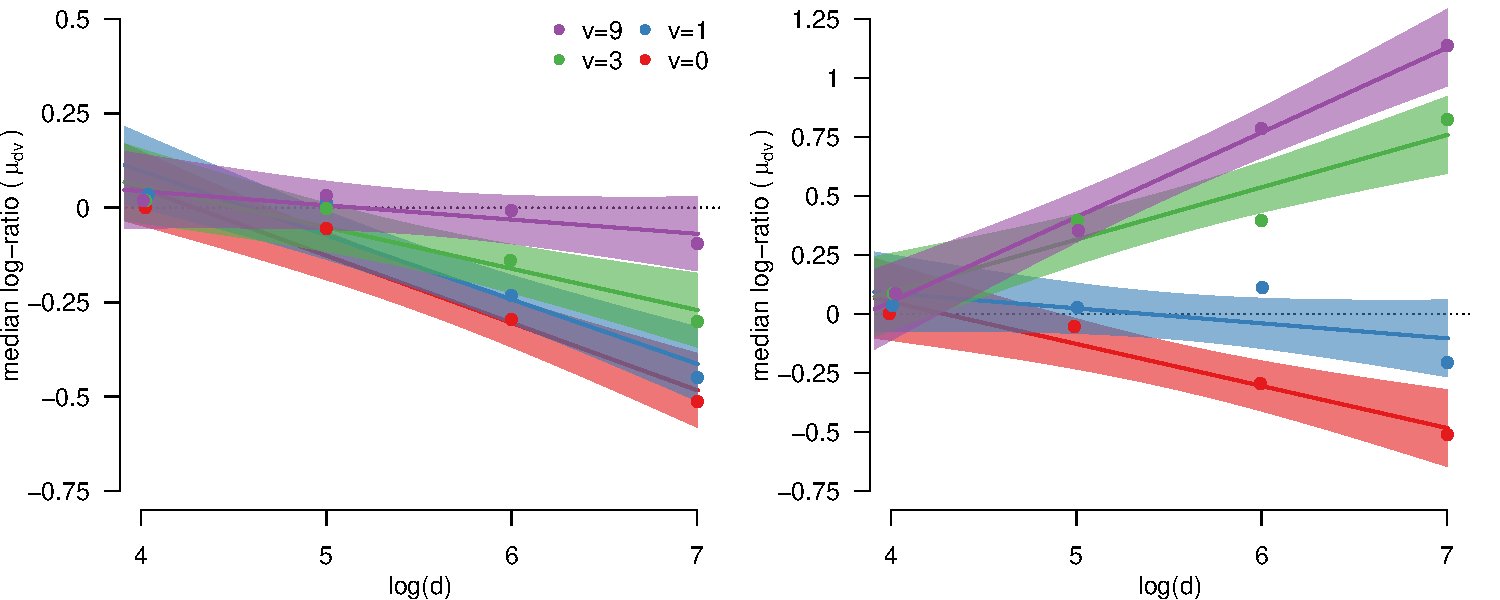
\includegraphics[width=1\linewidth]{medians.pdf}
	\caption{\footnotesize \textbf{Thread accuracy}. Relationship between median log-ratio $y_{dv}$ and $\log(d)$ with 95\% confidence bounds (shaded areas) in pristine, historical threads \textbf{(left)} and manipulated threads \textbf{(right)}. Colors represent the number of visible estimates, $v$. There is a clear relation between $d$ and $v$ showing that social information plays a dual role in difficult tasks: When $v$ is large, pristine and unmanipulated social information \textbf{(left)} counteracts underestimation bias and improves thread accuracy. When the social information is manipulated \textbf{(right)}, however, a strong overestimation bias emerges for large $v$. The red lines, corresponding to the control groups with $v=0$, are identical in both plots.}
	\label{fig:medians}
\end{figure*}


We also propose the experimental mechanism of dot-guessing games \cite{horton2010dot}, where participants guess the number of dots in an image. While dot estimations have been used previously in numerosity experiments \cite{minturn1951effect, indow1977scaling, krueger1982single} they have only recently been proposed as useful ‘model organisms’ for crowd aggregation research \cite{horton2010dot, ugander2015wisdom} due to their advantages in terms of cultural neutrality, resistance to expertise and/or prior knowledge, and their qualities as captchas \cite{von2008recaptcha}. In addition, dot estimation tasks are easy to implement and easy to understand. Most importantly, they have an objective solution and are tunable, allowing for nearly-continuous difficulty levels and performance measures.



%\section*{Experimental Design}
We collected a total of 11,748 estimates from 6,196 unique participants on Amazon Mechanical Turk. 5,990 estimates were collected from participants placed in 12 different threads where they successively estimated the number of dots, $d \in \{55,148,403,1097\}$, in an image, while seeing the $v \in \{1,3,9\}$ \textit{preceding} estimates (historical threads). Another 3,934 estimates were collected from participants who were placed in 12 other threads and shown the same images while seeing the $v \in \{1,3,9\}$ \textit{highest} estimates made so far (manipulated threads). Finally, 1.824 estimates were collected from participants who were shown the same images, but with $v=0$, corresponding to control conditions for each $d$ containing no social information.

We interpret the number of dots, $d$, as the \textit{task difficulty}, while the number of visible previous estimates, $v$, is interpreted as the \textit{degree of social information}. Participants were placed randomly in one of the 28 threads ($2 \times 3 \times 4$ + 4 controls)  and made their estimate one after another. In order to keep the estimates in a somewhat realistic range, participants could not submit numbers below 10 and above 1.000.000. No participant who had seen a certain image would be able to participate in another thread containing the same image again. In addition to a participation fee and a variable waiting fee, all participants in all threads received a bonus of \$1 if their estimate was within 10\% of the true value. See the Methods section and the Supplementary Information for additional information about the experimental design.

%\section*{Methods}
Free response elecitation of absolute values is known to create right-skewed distributions with long tails, which inflate the means. While it is still debated which measure is best suited to aggregate such data \cite{kao2018counteracting}, we follow the lead of Galton \cite{galton1907vox} and focus on the median as it is easy to interpret, robust against outliers, and best expresses the opinion of the crowd in the sense that the majority deems every other estimate as too high or too low. For the statistical analysis of thread aggregates, we therefore compare the log-ratio of thread medians, $y_{dv}=\log(M_{(d,v)}/d)$, using a linear normal model to quantify differences between threads in terms of $\log(d)$ and $v$, the latter as a categorical variable. The effects of social information on individual descision-making are analysed using a GMM on the log-ratio of individual estimates $Y_i$ with the weighted geometric mean of the social information as the explanatory variable. %Model dependecies are shown in Figure~\ref{fig:model}.
The model assigns a \textit{persuadability score}, $\beta^w$, to each participant, which is high when people are highly influenced by the social information they can see, and small when people are not influenced, or when they are skeptical about the information (see Methods for details).

\subsection*{Results}
\begin{figure*}[h]
	\centering
		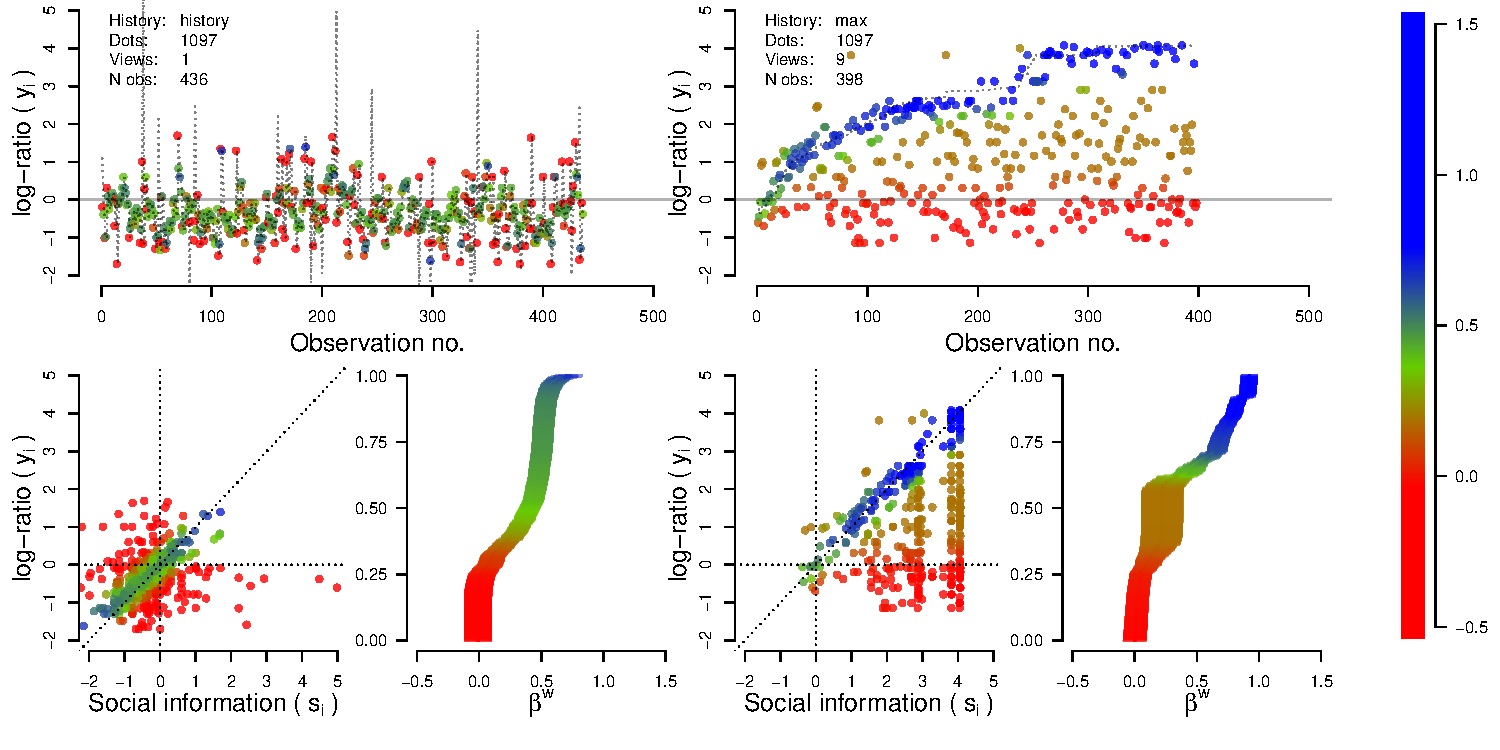
\includegraphics[width=1\linewidth]{threads.pdf}
		\caption{\footnotesize \textbf{GMM results:} The left hand side shows three plots of a historical thread with $d=1097$ and $v=1$, and the right hand side shows three plots of a manipulated thread with $d=1097$ and $v=9$. Top plots show the log-ratio estimates over time (observation no.), with the weighted geometric mean of the social information shown by a dotted line. Bottom left plots show the log-ratio of the estimates as a function of the log-ratio of the social information, indicating how differently participants use their social information. Bottom right plots show the cumulative distribution of individual persuadability scores with 95\% intervals derived from the fitted models.}
\label{fig: social influence}
\end{figure*}

In accordance with previous findings, participants do well in tasks without social information, especially when estimating small numbers. For higher difficulties estimates vary widely and biases become substantial \cite{indow1977scaling, izard2008calibrating, krueger1982single, krueger1984perceived, kao2018counteracting}. The median tends to underestimate the true value and the mean tends to overestimate the true value. %Summary statistics of all 28 treatments can be inspected graphically and in table format in the supplementary information (SI).

\subsubsection*{Analysis of thread performance}
The relationship between the observed median log-ratio $y_{dv}$ and the number of dots $d$ are found suitable, according to quantile-quantile plots (see SI-text), when modeling $y_{dv}$ against $\log{d}$ and $v$. %We thus quantify the overall differences between threads in terms of the log-ratio of their medians, $y_{dv}$, as a function of $\log(d)$ and $v$. 
For more details, see the Methods section. Historical and manipulated threads are modelled separately to allow for differing error variances.

Figure \ref{fig:medians} (left) shows that the collective performance of historical threads declines significantly with increasing task difficulty $d$, but improves with the amount of social information. In contrast to \cite{lorenz2011social, king2011true, minson2012cost} and in concert with \cite{gurccay2015power, becker2017network, jayles2017social, farrell2011social} these findings support the claim that crowds indeed may become wise under (pristine) social influence. It should be noted, however, that the overlapping confidence intervals reveal where thread performances are comparable. Thus, the negative effects of task difficulty and the positive effects of social information are only discernible in situations where people have hard problems to solve, and at the same time have social information in abundance. In fact, the median estimate of historical threads with $v=9$ is `wise' in the sense of being statistically indistinguishable from the true value for all $d$.

In manipulated threads, Fig.\ref{fig:medians} (right), the manipulation results in a large positive bias for $v=3,9$ which increases with $d$, implying that when a task becomes more demanding, the amount of (filtered) social information has a highly detrimental impact on thread performance. For $v=1$ there is still a small negative trend, implying that the manipulation is not very effective. This resonates well with the findings in \cite{jayles2017social} which shows that providing a moderate amount of incorrect information may counterbalance underestimation bias and improve collective performance.

\subsubsection*{Analysis of Persuadability}
% A GMM is fitted to all threads after removing estimates below the 2.5\% and above the 97.5\% quantiles. For each model, standardized residuals are evaluated visually using quantile-quantile plots against a standard normal $\mathcal{N}(0,1)$, see Supplementary Information. These plots reveal that models using $k=2,3,4$ states fit the data quite well, with only a few models displaying a less adequate fit.  (repetition from Methods)

In Fig. \ref{fig: social influence} two exemplary threads show how the GMM model framework reveals interesting features of the data. Each thread is represented by three figures. The top figures show the log-ratio of estimates as the thread evolves over time with the weighted geometric mean of the social information shown by a dotted line. Each estimate has an associated color, given by the persuadability score $\beta^w$, which measures the influence of social information on each participant. A high value ($\beta^w>0.6$) in dark green and blue colors implies a large social influence effect, a low value ($\beta^w\approx 0$) in red implies a small or no effect, and a medium value ($\beta^w \approx 0.4$) in brown and light green colors suggests a compromise between the two extremes. The RGB color scale (right) is the same for all threads and plots. The bottom left plots show the log-ratio of the estimates as a function of the log-ratio of the social information, indicating how differently people use their social information: The more they align with the identity line, the more they tend to follow the social information.

\begin{figure*}[!h]
	\centering
	\hspace{-30px}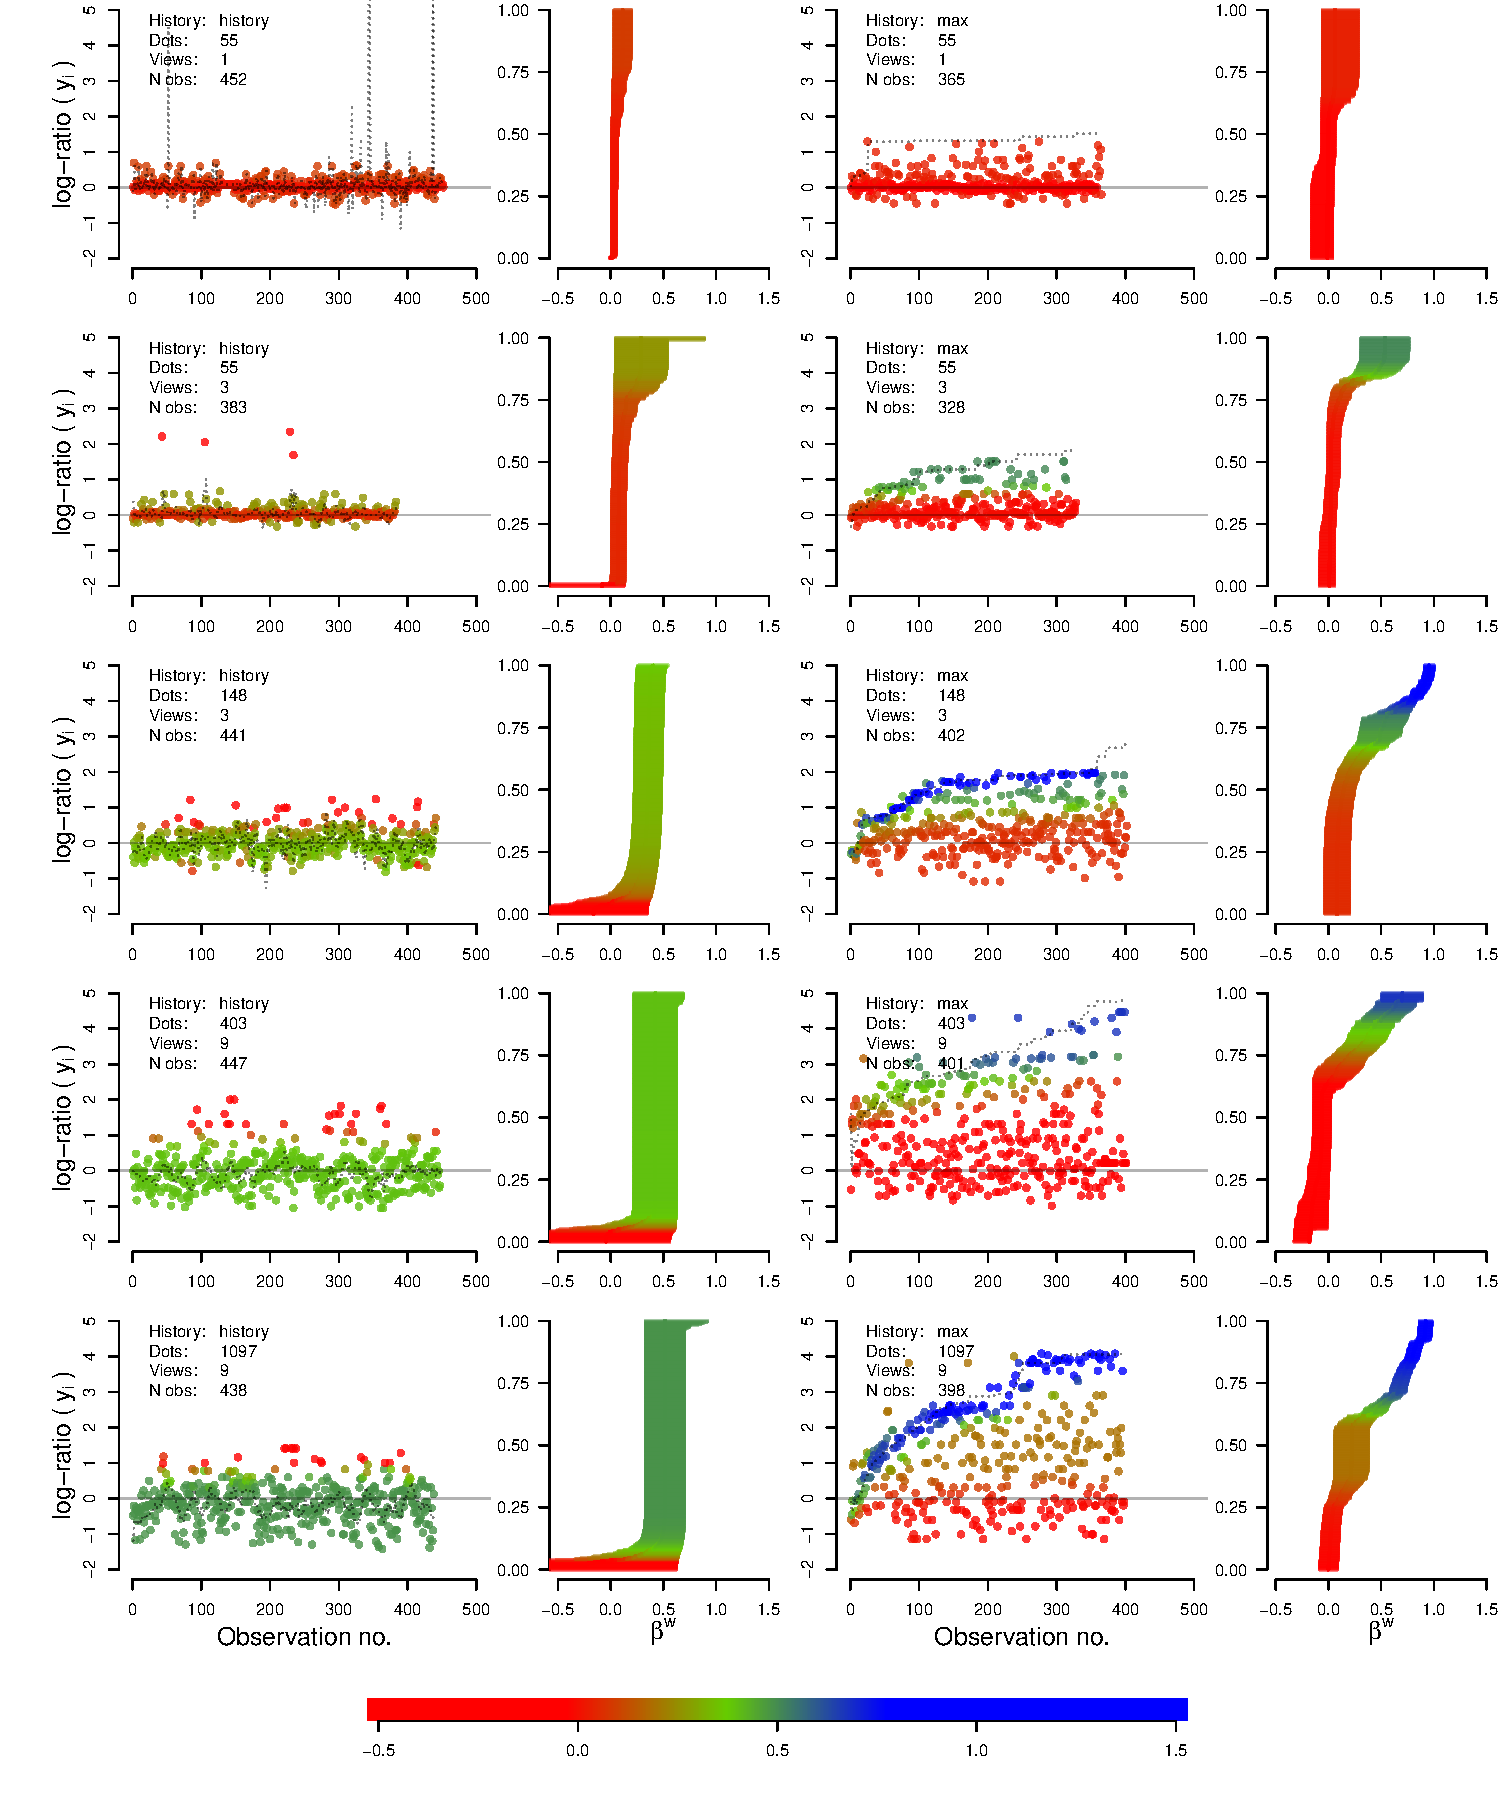
\includegraphics[width=1\linewidth]{thread_evolution}
	\caption{\footnotesize \textbf{Thread dynamics:} Comparison of typical historical threads (left) and their corresponding manipulated versions (right).
	Colors correspond to estimated $\beta^w$ values. The color scale is fixed across threads.}
\label{fig:more}
\end{figure*}

The bottom right plots show the cumulative distribution of the persuadability scores with 95\% confidence intervals derived from the fitted model. They clearly show how people may be categorized into those ‘sleeping dogs’ or ‘lost causes’ \cite{devriendt2018literature} in red that do not take other peoples estimates into account, the `persuadables' that tend to follow others, and a large group of green `compromisers', who try to strike a balance between what they see others have guessed, and what they believe themselves. Of course, such labels are only proximate. Given a participant has a personal estimate much in line with the social information seen, this participant may be labelled as a persuadable or as a compromiser, when in fact this is only partially true. In general, however, the distributions are remarkable stable across threads, which suggests that people indeed may be partitioned into such overlapping response types.


\subsubsection*{Thread dynamics}
What becomes abundantly clear when examining the results from the GMMs, is a sharp contrast between how people act in pristine historical threads, and how people act in manipulated, filtered threads. This is shown in Figure~\ref{fig:more}, where we compare typical historical threads (left) with their corresponding manipulated treatments (right). When the task difficulty is low and $v=1$, participants are not significantly influenced, no matter whether they see the preceding or highest estimate in their thread (top row in Figure~\ref{fig:more}). But as soon as the amount of social information increases (second row), more people tend to follow – or at least to compromise. This indicates that there is a bandwagon effect at work \cite{bikhchandani1992theory, lee2018understanding}, making it more likely for people to follow others, the more people have done so already. 

If we increase the difficulty of the task from $d=55$ to $d=148$ and keep $v$ constant at $v=3$, as shown in the third row of Figure~\ref{fig:more}, the dynamics between the historical thread on the left diverges strongly from the dynamics of the manipulated thread on the right. While the majority of participants in the historical thread are easier to persuade (green colors), people in the manipulated thread become more diverse and slowly start to split bewteen those, who are highly persuadable (blue) and those who are not (red). Increasing difficulty even further to $d=403$, and also increasing the amout of social information to $v=9$, as shown in the fourth row of Figure~\ref{fig:more}, makes this split in behaviour even more visible. For $d=1097$ and $v=9$, as shown in the bottom row, the difference is very clear: In the historical thread, a large majority of participants are medium to strongly influenced, having a persuadability score around $0.5$, probably because most of the social information they see is regarded as more or less reasonable. However, as can be seen in the $\beta^w$-distribution, there is a high uncertainty in the scores, because we only model the weighted geometric mean of the nine preceding estimates, while people presumably are much more diverse in the way they process these estimates.


%In the following, we dive deeper into the results from the GMM's. In the main text we established that when task difficulty is low and $v=1$, participants are not significantly influenced, no matter whether they see the preceding or highest estimate in their thread. But as soon as $v$ increases, more people tend to follow – or at least compromise on what the see other participants have estimated, and what they believe themselves.

%In Figure~\ref{fig:more} . In the top row we have threads with $d=55$ and $v=1$. Both shown only in red colors, indicating that participants are not influenced by the single other estimate they can see, probably because it is easy for people to see that the actual number of dots in the image is in the range of 50-60. The next row shows the historical and manipulated threads with $d=55$ and $v=3$. Even though the task difficulty is held constant, green colors appear, implying that more people tend to follow – or at least to compromise – upon their own estimates. %This shows that there is a bandwagon effect at work, making it more likely for people to follow others the more people have done so already.

\subsection*{Discussion}
Returning to the initial question of whether social information helps crowd wisdom, or whether it does more harm than good, our answer is both. Social information in online estimation threads does help when people have difficult questions to answer and when the information available to them is pristine and therefore representative. However, if the social information is filtered and not representative of the thread population, it becomes manipulative and may fool a substantial proportion of people, which, of course, interferes with any aspiration to harness the powers of collective intelligence.

Moving from the aggregate to the individual level, we find that people can be assigned a persuadability score by using a Gaussian Mixture Model. Persuadability generally increases with task difficulty and with the amount of social information provided. In the case of strong manipulation, we may see a split between a minority of persuadables and a majority of compromisers and skeptics. We do not know how much these influencing effects are transferable to other domains. However, due to the general nature of dot estimations, we suspect the effects to be substantial in other settings as well, and also for other questions – especially for those that are more emotional, subjective and political in nature. In computational social science and decision-making research,  there is an acute need to further investigate the types of ‘disturbances’ in online threads and crowds, such as filters, rankings, likes, and recommendations, as well as the types of reaction to those disturbances. To the end of designing future collective intelligence systems, one needs to be vigilant about the way social information is gathered and framed. Crowd knowledge and thread wisdom is fragile, and can only be maintained with strong controls upon the way it is cultivated and recovered.

\subsection*{Methods}\scriptsize
\subsubsection*{Experimental design and data collection}
All experiments were coded in otree 2.1 \cite{chen2016otree}. The code itself is designed along the same lines as the classical information cascade experiments by Anderson and Holt \cite{anderson1997information}. A participant makes an estimate, and the next one receives the information about the estimate of the previous participant(s). %Thus, the main technical issue is that only one person at a time can make a decision while others wait. As soon as a participant finishes and leaves the choice page, the next participant enters while all subsequent participants still have to wait.
We obtained a total of 11.748 estimates from 6.196 unique participants. Any dot-image was only seen once by a participant, i.e. we had a total of 3.157 participants seeing only one image, 1.259 participants seeing two images, 1.047 participants seeing three images, and 733 participants seeing all four images (either in the unmanipulated or manipulated conditions and with $v \in \{0, 1, 3, 9\}$). After providing informed consent, participants waited in a ‘waiting room’ until the ‘choice room’ became available. When entering the choice room participants could see an image $d$ together with $v \in \{0,1,3,9\}$ previous estimates. After making an estimate, participants were thanked and paid a participation fee of \$0.10 and bonus of \$1 if their estimate was within 10\% of the true number. The average time used was less than two minutes, see SI-text for screenshot and detailed design descriptions.

\subsubsection*{Analysis of thread medians} For the observed medians $M_{dv}, d\in \{55,148,403,1097\}, v \in \{0,1,3,9\}$ the log ratios $y_{dv} = \log (M_{dv}/d)$ were modeled using a linear normal model. For a given thread, $\log{d}$ was used as a quantitative variable whereas $v$ was used as a categorical factor. Hence, the model structure for the medians was $\mu_{dv} = \alpha_v+\beta_v\log{d}$. Models were fitted separately to historical and manipulated threads to allow for different variance estimates $\hat{\sigma}^2$ between these groups. Goodness of fit was assessed by quantile-quantile (QQ) plots of the residuals (see SI-text, Figure~\ref{fig: qq plots median}). Although some deviation is present, with the available number of observations we do not discard the models based on these plots. The low number of observations also implies wide confidence bands, hence conclusions from the models can be viewed as conservative.

%\section*{Statistical methods}
%\subsection*{Analysis of thread medians}
%The medians were modeled as a linear normal models for the history and manipulated series separately, where the mean in each case was specified as
%\begin{align*}
%	\mu_{dv} = \alpha_v+\beta_v\log(d), \quad d=55, 148, 403, 1097, \enskip v=0,1,3,9 .
%\end{align*}
%The number of views was treated as categorical, since there were clearly an effect of different views, but it was hard to quantify the relationship between different number of views. The ($\log$) number of visible dots was modeled as a quantitative variable, since the distance between $\log(d)$ were deemed suitable scores for this variable, especially since the number of dots were chosen as $e^{\delta}, \delta=4,5,6,7$ rounded to nearest integer. The quantitative nature of $d$ was also chosen to lower the number of variables in the model, due to the low number of observations (medians) available.
%
%The models were assessed by quantile-quantile (QQ) and residual plots, as shown in Figure~\ref{fig: qq plots median}. Although some deviation is present, with the available number of observations we do not discard the models based on these plots. The low number of observations also implies wide confidence bands, hence conclusions from the models can be viewed as conservative.

\subsubsection*{GMM model for social influence}
A Gaussian Mixture Model (GMM) was used to cope with the heavy tails and skewness present in the data. The GMM employs a fixed number of states to fit a weighted sum of Gaussian distributions to each observation, hence the \emph{mixture} labeling.

Let $X_i=\{1,\dots,k\}$ denote the state variable and $Y_i$ the observation for participant $i=1,\dots,n$. Then, conditional on $X_i=j, j=1,\dots,k$, $Y_i$ follows a normal distribution
\begin{align*}
	Y_i|(X_i=j)  \sim \mathcal{N} (\mu_j,\sigma^2_j), j=1,\dots,k,
\end{align*}
hence the unconditional distribution of $Y_i$ is obtained by integrating (i.e. summing since $X_i$ is discrete) over $X_i$
\begin{align*}
	P(Y_i) = \sum_{j=1}^k P(X_i=j)P(Y_i|X_i=j).
\end{align*}
Including social information as an observed variable in the model, $Y_i$ depends on both $X_i$ and $S_i$, if $v>0$. Furthermore, if $v>0$, then $Y_i$ influences $S_{i+1}$ as the next participant $Y_{i+1}$ will see the estimate of $Y_i$ (assuming the history provided is the previous views). A graphical presentation of model dependencies (with preceding views available) are shown in Figure~\ref{fig:model}.

\begin{figure}[!h]
\centering
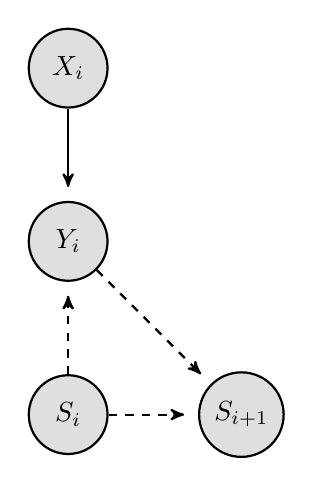
\begin{tikzpicture}[->,>=stealth',shorten >=5pt,auto,node distance=2.2cm, thick,main
node/.style={circle,fill=gray!25,draw,font=\sffamily\bfseries, minimum size=1cm}]
	\node[main node] (x1) {$X_{i}$};
	%\node[main node] (x2) [right of=x1] {$X_{i+1}$};
	\node[main node] (y1) [below of=x1] {$Y_{i}$};
	%\node[main node] (y2) [below of=x2] {$Y_{i+1}$};
	\node[main node] (m1) [below of=y1] {$S_{i}$};
	\node[main node] (m2) [right of=m1] {$S_{i+1}$};
	\path[every node/.style={font=\sffamily\small}]
    		%(m1) edge [dashed, bend right=30] (m2)
    		(m1) edge [dashed] (m2) edge [dashed] (y1)
		%(m2) edge [dashed] (y2)
		(y1) edge [dashed] (m2)
		(x1) edge (y1)
		%(x2) edge (y2)
  		;
	\end{tikzpicture}
	\caption{\tiny Gaussian Mixture Model dependencies with the observed estimate $Y_i$ by participant $i$, the latent state variable $X_i$, and the social information $S_i$ when consisting of preceding estimates. Dashed lines are connections that depend on the number of views $v$. When $v=0$, $S_i$ is omitted from the model, when $v=1$ then $S_i\to Y_i$ and $Y_i\to S_{i+1}$. For $v>1$ then $S_i\to S_{i+1}$ is added.}
\label{fig:model}
\end{figure}

Thus, given $k$ independent states and using $\delta_{ij} = P(X_i=j)$, then $Y_i$ is normally distributed with parameters
\begin{align}
\begin{array}{l}
	\mu^w_i = \sum_{j=1}^k \delta_{ij} \mu_j \\
	(\sigma^w_i)^2 = \sum_{j=1}^k \left(\delta_{ij} \sigma_j\right)^2
\end{array}
\quad i=1,\dots,n \label{eq: weighted Gaussian parameters}
\end{align}
where the mean $\mu_j$ is modeled with social information $s_i$ as
\begin{align}
	\mu_j = \alpha_j+\beta_j s_i, \quad i=1,\dots,n, j=1,\dots,k.
\end{align}
Note that $\mu^w_i$ and $\sigma^w_i$ refer to the weighted estimates, unique to each observation $y_i, i=1, \dots, n$. This implies, that the effect of social information becomes a weighted sum of $\beta_j$ estimates
\begin{align}
	\beta^w_i = \sum_{j=1}^k \delta_{ij} \beta_{j}, \quad i=1,\dots, n. \label{eq: weighted beta}
\end{align}
Similarly for the $\alpha_i^w$ parameter, modeling the accompanying intercept.

It should be emphasized that the weighted $\alpha_i^w,\beta_i^w$ are unique for each observation due to the weights $\delta_{ij}$, contrary to a standard regression model where all observations are assumed to adhere to the same effects. For the GMM this can be interpreted as each participant is modeled as a weighted average of $k$ strategies. Hence, the personal strategy is unique, due to $\delta_{ij}$, but weighted among $k$ general dimensions.

For each model, the number of states were set to $k=2,3,4,5$ and the model with the lowest Bayesian Information Criteria (BIC) was chosen as the preferable one. The BIC was used rather than the more usual Akaikes Information Criteria (AIC), since the BIC penalized the number of parameters more heavily. The aim was to settle with a decent model fit, with fewer parameters to avoid overfitting. 
In our case AIC: $6k-2\ln(L)$ and BIC: $3k\ln(n)-2\ln(L)$, where $L$ refers to the likelihood value. Note that both criteria are scaled with $3k$ parameters for $k$ states. The BIC penalizes the number of parameters weighted by the ($\log$) number of observations $n$,
as $3k$, corresponding to $(\delta_i,\mu_i,\sigma^2_i)$ for each state, whereas AIC only penalizes by a factor 2. 
Using objective criteria to choose a number of states/clusters is often prone to simply increase $k$ continuously \cite{hastie2009} and as such the AIC yielded much larger $k$ values ($k \gg 5$), practically implying that $k=5$ for all models, due to us capping this parameter at this value. This effect was not seen for the BIC measure for $2\leq k \leq 5$, further supporting this choice of objective measure.
% Tibshirani, Elements of Statistical Learning section 14.3.11


The goodness of fit for the GMM was assessed by calculating standardized residuals
\begin{align}
 	\hat{\varepsilon}_i = \frac{y_i - \hat{\mu}^w_i}{(\hat{\sigma}^w_i)^2} = (y_i - \hat{\alpha}^w_i-\hat{\beta}^w_ix_i)/(\hat{\sigma}^w_i)^2 \label{eq: GMM residuals}
\end{align}
and assessing the empirical distribution of $\hat{\varepsilon}_i, i=1,\dots,n$ against a standard $\mathcal{N}(0,1)$ distribution.

After removing the 5\% most extreme observations, i.e. estimates below the 2.5\% and above the 97.5\% thresholds, Fig. \ref{fig: QQ plots AMT} in the SI-text shows the QQ-plots of the fitted models. Fig. \ref{fig: weighted beta distributions} in the SI-text shows the estimated $\hat{\beta}^w$ distributions, with 95\% confidence bounds provided by the models. Fig. \ref{fig: threads with social info and colored by beta weights} in the SI-text shows the observed threads, colored by the individual $\hat{\beta}^w$ values, and the available social information. Fig. \ref{fig: social info vs estimates} shows the observed estimates against the available social information, again colored by their individual $\hat{\beta}^w$ values.

\subsubsection*{Modeled values}
The observations in the model were transformed to achieve a better fit. The estimates were standardized with the relevant number of dots and then $\log$-transformed. Hence, for an observed estimate $e_i$ on $d$ dots
\begin{align*}
	y_i = \log(e_i/d), \quad i=1,\dots,n.
\end{align*}
The available social information, $s_i$, available for participant $i$ in a given thread was modeled as an aggregated value of the available previous estimates. If we let $z_{i,\{1,\dots,v\}}$ denote these $v$, then for the un-manipulated threads $z^h_{i, \{1,\dots,v\}} = \{e_{i-1},\dots,e_{i-v}\}$ and for the manipulated threads $z^m_{i, \{1,\dots,v\}} = \{e^*_{(1)},\dots,e^*_{(v)} | e^*_j=e_j, j<i\}$, where $e^*_{(1)}\geq e^*_{(2)}\geq\dots\geq e^*_{(v)}\geq e^*_{(l)}$ denote the (decreasingly) ordered estimates $e^*_j$ among $e_1,\dots,e_j$, for $v<l\leq j<i$. The superscripts $h,m$ refer to the type of information available, either historical ($h$) or manipulated ($m$). Hence, the historical information are the preceding $v$ estimates, whereas the manipulated information are the $v$ largest estimates among all preceding estimates. \\
Following \citep{jayles2017social} the aggregation of these estimates was a weighted geometric mean. However, contrary to \citep{jayles2017social}, the actual estimates were available to the participants, hence in this context $s_i$ becomes a proxy for the available social information. Letting $z_{ij}$ denote the $j$'th visible estimate for the $i$'th participant in either type of threads, then
\begin{align*}
	s_i = \log\left(\frac{\prod_{j=1}^v z_{ij}^{w_j}}{d}\right) %= \sum_{j=1}^v w_j \log(g^\text{pre}_j)-\log(d)
	= \sum_{j=1}^v w_j \log\left(\frac{z_{ij}}{d}\right),
\end{align*}
where $\sum_{j=1}^v w_j = 1$. Thus, the log-transform implies that the modeled values (log-normalized estimates) are aggregated as a simple weighted mean. The pair $(y_i,s_i), i=1,\dots,n$ were then used in the GMM framework. The weights $w_j, j=1,\dots,v$ were determined from density estimates based on the control threads of $v=0$. Hence, for $d$ dots, a density was estimated from the $v=0$ thread and then used as a proxy for how individuals in a thread with $v>0$ would estimate without any social information. Using this, an individual in a thread with $v>0$ is then assumed to assess the available previous estimates based on this density. This way extreme estimates are naturally filtered and a participants information is therefore almost exclusively weighted among sensible estimates. Practically this implied that estimates within boundaries considered extreme, were almost equally weighted, however extreme inputs, either by deliberate efforts to mislead the thread or otherwise just to be considered nuisances were weighted almost at 0, yielding a more reasonable aggregated social information input $s_i$. For manipulated threads, or threads with $v=1$, the social information available show these extreme guesses. This is simply what a participant have seen and will thus be discarded by the parameter estimation, fitting a low $\beta^w$ value for this participant (assuming that the current participant submits a realistic estimate and not taking the extreme info into account). In the case of manipulated threads, due to the removal of most extreme estimates to filter out deliberate extremities, the social information available can be higher than the cutoff limit of the 97.5\% quantile. However, as in the case of $v=1$, this will simply be the available information that a participant can follow or disregard. The model will thus fit a suitable $\beta^w$ value based on the current participants use of the info available. The R package \texttt{depmixS4} \cite{visser2010} was used to fit the model, using an EM algorithm to maximize the log-likelihood function of the model.

%\subsubsection*{Analysis of social influence}
%The influence of social information was analyzed using a Gaussian Mixture Model (GMM) for each individual thread. The flexibility of these models allow for heavier tails and skewness present in the in the data. Individual estimates $e_i$ are transformed as the log-ratio relative to the true number of dots in order to compare threads of differing difficulty. Therefore,
%\begin{align}
%	y_i = \log(e_i/d), i=1,\dots,n. \label{eq: y values for gmm}
%\end{align}
%The social influence variable $s_i, i=1,\dots, n$ was calculated as a weighted geometric mean of previous estimates, with the weighting derived from density estimates of the control groups with $v=0$. The geometric mean follows the idea of \citep{jayles2017social} where the authors argue that a multiplicative aggregation is more inline with human behavior. The relative social information was also log-transformed analogously with Eq. \ref{eq: y values for gmm}.  For a GMM with $k$ states, each state model then becomes
%\begin{align}
%	\mu_j = \alpha_j+\beta_j s_i \quad, i=1,\dots,n, j=1, \dots,k. \label{eq: mean models}
%\end{align}
%The number of states, $k$, was chosen by the associated Bayesian Information Criteria (BIC), but was capped at $k=5$. For each observation $y_i$, each state is assigned a weight $\delta_{ij}$, such that the $i$'th mean is a weighted sum
%\begin{align}
%	\mu^w_i = \sum_{j=1}^k\delta_{ij}\mu_j = \sum_{j=1}^k\delta_{ij}(\alpha_j +\beta_j s_i),
%\end{align}
%where
%\begin{align}
%	\beta^w_i = \sum_{j=1}^k \delta_{ij}\beta_j, \quad i=1,\dots, n, j=1,\dots,k \label{eq: weighted beta}
%\end{align}
%is the estimated influence of social information which we denote the \emph{persuadability score} of the $i$'th participant in the thread. It should be emphasized that the weighted $\beta^w_i$ is unique for each observation due to the weights $\delta_{ij}$, contrary to a standard regression model where all observations are assumed to adhere to the same $\beta$-effect. For the GMM, this can be interpreted as each participant being modeled as a weighted average of $k$ strategies. Hence, the personal strategy is unique, due to $\delta_{ij}$, but weighted among $k$ general dimensions. The goodness of fit for the GMM was assessed by visualizing the residuals (see SI-text).

\subsection*{Reporting Summary.}\footnotesize Further information on research design is available in the Nature Research Reporting Summary linked to this article..

\subsection*{Data availability}\footnotesize Anonymized datafile ``dots.csv'' can be downloaded at (blinded). Parameters: task = type of experiment; $d$ = number of dots in image; $v$ = number of visible preceding estimates; session = thread name; hashed\_turker = anonymized participant id; decision order = order in which participants enter the queue; hist = list of guesses seen by participant; guess = estimate by participant

\subsection*{Code availability}\footnotesize The replication files for this paper, including the Python and R code associated with all calculations and plots are available on github/(blinded).



% Bibliography (hand made)

\setlength{\bibsep}{0.0pt}
%\bibliographystyle{naturemag}
%\bibliography{wamot}

\begin{thebibliography}{10}
\expandafter\ifx\csname url\endcsname\relax
  \def\url#1{\texttt{#1}}\fi
\expandafter\ifx\csname urlprefix\endcsname\relax\def\urlprefix{URL }\fi
\providecommand{\bibinfo}[2]{#2}
\providecommand{\eprint}[2][]{\url{#2}}

\bibitem{woolley2010evidence}
\bibinfo{author}{Woolley, A.~W.}, \bibinfo{author}{Chabris, C.~F.},
  \bibinfo{author}{Pentland, A.}, \bibinfo{author}{Hashmi, N.} \&
  \bibinfo{author}{Malone, T.~W.}
\newblock \bibinfo{title}{Evidence for a collective intelligence factor in the
  performance of human groups}.
\newblock \emph{\bibinfo{journal}{Science}} \textbf{\bibinfo{volume}{330}},
  \bibinfo{pages}{686--688} (\bibinfo{year}{2010}).

\bibitem{gurccay2015power}
\bibinfo{author}{G{\"u}r{\c{c}}ay, B.}, \bibinfo{author}{Mellers, B.~A.} \&
  \bibinfo{author}{Baron, J.}
\newblock \bibinfo{title}{The power of social influence on estimation
  accuracy}.
\newblock \emph{\bibinfo{journal}{J Behav Decis Making}}
  \textbf{\bibinfo{volume}{28}}, \bibinfo{pages}{250--261}
  (\bibinfo{year}{2015}).

\bibitem{becker2017network}
\bibinfo{author}{Becker, J.}, \bibinfo{author}{Brackbill, D.} \&
  \bibinfo{author}{Centola, D.}
\newblock \bibinfo{title}{Network dynamics of social influence in the wisdom of
  crowds}.
\newblock \emph{\bibinfo{journal}{P Natl Acad Sci Usa}}
  \textbf{\bibinfo{volume}{114}}, \bibinfo{pages}{E5070--E5076}
  (\bibinfo{year}{2017}).

\bibitem{jayles2017social}
\bibinfo{author}{Jayles, B.} \emph{et~al.}
\newblock \bibinfo{title}{How social information can improve estimation
  accuracy in human groups}.
\newblock \emph{\bibinfo{journal}{P Natl Acad Sci Usa}}
  \textbf{\bibinfo{volume}{114}}, \bibinfo{pages}{12620--12625}
  (\bibinfo{year}{2017}).

\bibitem{caplan2011myth}
\bibinfo{author}{Caplan, B.}
\newblock \emph{\bibinfo{title}{The Myth of the Rational Voter: Why Democracies
  Choose Bad Policies-New Edition}} (\bibinfo{publisher}{Princeton University
  Press}, \bibinfo{year}{2011}).

\bibitem{lorenz2011social}
\bibinfo{author}{Lorenz, J.}, \bibinfo{author}{Rauhut, H.},
  \bibinfo{author}{Schweitzer, F.} \& \bibinfo{author}{Helbing, D.}
\newblock \bibinfo{title}{How social influence can undermine the wisdom of
  crowd effect}.
\newblock \emph{\bibinfo{journal}{P Natl Acad Sci Usa}}
  \textbf{\bibinfo{volume}{108}}, \bibinfo{pages}{9020--9025}
  (\bibinfo{year}{2011}).

\bibitem{minson2012cost}
\bibinfo{author}{Minson, J.~A.} \& \bibinfo{author}{Mueller, J.~S.}
\newblock \bibinfo{title}{The cost of collaboration: Why joint decision making
  exacerbates rejection of outside information}.
\newblock \emph{\bibinfo{journal}{Psychol Sci}} \textbf{\bibinfo{volume}{23}},
  \bibinfo{pages}{219--224} (\bibinfo{year}{2012}).

\bibitem{king2011true}
\bibinfo{author}{King, A.~J.}, \bibinfo{author}{Cheng, L.},
  \bibinfo{author}{Starke, S.~D.} \& \bibinfo{author}{Myatt, J.~P.}
\newblock \bibinfo{title}{Is the true ‘wisdom of the crowd’to copy
  successful individuals?}
\newblock \emph{\bibinfo{journal}{Biol Lett}} \textbf{\bibinfo{volume}{8}},
  \bibinfo{pages}{197--200} (\bibinfo{year}{2011}).

\bibitem{le2018endogenous}
\bibinfo{author}{Le~Mens, G.}, \bibinfo{author}{Kov{\'a}cs, B.},
  \bibinfo{author}{Avrahami, J.} \& \bibinfo{author}{Kareev, Y.}
\newblock \bibinfo{title}{How endogenous crowd formation undermines the wisdom
  of the crowd in online ratings}.
\newblock \emph{\bibinfo{journal}{Psychol Sci}} \textbf{\bibinfo{volume}{29}},
  \bibinfo{pages}{1475--1490} (\bibinfo{year}{2018}).

\bibitem{salganik2006experimental}
\bibinfo{author}{Salganik, M.~J.}, \bibinfo{author}{Dodds, P.~S.} \&
  \bibinfo{author}{Watts, D.~J.}
\newblock \bibinfo{title}{Experimental study of inequality and unpredictability
  in an artificial cultural market}.
\newblock \emph{\bibinfo{journal}{Science}} \textbf{\bibinfo{volume}{311}},
  \bibinfo{pages}{854--856} (\bibinfo{year}{2006}).

\bibitem{salganik2009web}
\bibinfo{author}{Salganik, M.~J.} \& \bibinfo{author}{Watts, D.~J.}
\newblock \bibinfo{title}{Web-based experiments for the study of collective
  social dynamics in cultural markets}.
\newblock \emph{\bibinfo{journal}{Top Cogn Sci}} \textbf{\bibinfo{volume}{1}},
  \bibinfo{pages}{439--468} (\bibinfo{year}{2009}).

\bibitem{galton1907vox}
\bibinfo{author}{Galton, F.}
\newblock \bibinfo{title}{Vox populi (the wisdom of crowds)}.
\newblock \emph{\bibinfo{journal}{Cah Rev The}} \textbf{\bibinfo{volume}{75}},
  \bibinfo{pages}{450--451} (\bibinfo{year}{1907}).

\bibitem{muth1961rational}
\bibinfo{author}{Muth, J.~F.}
\newblock \bibinfo{title}{Rational expectations and the theory of price
  movements}.
\newblock \emph{\bibinfo{journal}{Econometrica}} \bibinfo{pages}{315--335}
  (\bibinfo{year}{1961}).

\bibitem{surowiecki2005wisdom}
\bibinfo{author}{Surowiecki, J.}
\newblock \emph{\bibinfo{title}{The wisdom of crowds}}
  (\bibinfo{publisher}{Anchor}, \bibinfo{year}{2005}).

\bibitem{hong2008some}
\bibinfo{author}{Hong, L.} \& \bibinfo{author}{Page, S.~E.}
\newblock \emph{\bibinfo{title}{Some microfoundations of collective wisdom}},
  \bibinfo{pages}{56--71} (\bibinfo{year}{2008}).

\bibitem{izard2008calibrating}
\bibinfo{author}{Izard, V.} \& \bibinfo{author}{Dehaene, S.}
\newblock \bibinfo{title}{Calibrating the mental number line}.
\newblock \emph{\bibinfo{journal}{Cognition}} \textbf{\bibinfo{volume}{106}},
  \bibinfo{pages}{1221--1247} (\bibinfo{year}{2008}).

\bibitem{nash2014curious}
\bibinfo{author}{Nash, U.~W.}
\newblock \bibinfo{title}{The curious anomaly of skewed judgment distributions
  and systematic error in the wisdom of crowds}.
\newblock \emph{\bibinfo{journal}{PLoS One}} \textbf{\bibinfo{volume}{9}},
  \bibinfo{pages}{e112386} (\bibinfo{year}{2014}).

\bibitem{kao2018counteracting}
\bibinfo{author}{Kao, A.~B.} \emph{et~al.}
\newblock \bibinfo{title}{Counteracting estimation bias and social influence to
  improve the wisdom of crowds}.
\newblock \emph{\bibinfo{journal}{J R Soc Interface}}
  \textbf{\bibinfo{volume}{15}}, \bibinfo{pages}{20180130}
  (\bibinfo{year}{2018}).

\bibitem{anderson1997information}
\bibinfo{author}{Anderson, L.~R.} \& \bibinfo{author}{Holt, C.~A.}
\newblock \bibinfo{title}{Information cascades in the laboratory}.
\newblock \emph{\bibinfo{journal}{Amer Econ Rev}} \bibinfo{pages}{847--862}
  (\bibinfo{year}{1997}).

\bibitem{bikhchandani1992theory}
\bibinfo{author}{Bikhchandani, S.}, \bibinfo{author}{Hirshleifer, D.} \&
  \bibinfo{author}{Welch, I.}
\newblock \bibinfo{title}{A theory of fads, fashion, custom, and cultural
  change as informational cascades}.
\newblock \emph{\bibinfo{journal}{J Polit Economy}}
  \textbf{\bibinfo{volume}{100}}, \bibinfo{pages}{992--1026}
  (\bibinfo{year}{1992}).

\bibitem{bakshy2015exposure}
\bibinfo{author}{Bakshy, E.}, \bibinfo{author}{Messing, S.} \&
  \bibinfo{author}{Adamic, L.~A.}
\newblock \bibinfo{title}{Exposure to ideologically diverse news and opinion on
  facebook}.
\newblock \emph{\bibinfo{journal}{Science}} \textbf{\bibinfo{volume}{348}},
  \bibinfo{pages}{1130--1132} (\bibinfo{year}{2015}).

\bibitem{banerjee1992simple}
\bibinfo{author}{Banerjee, A.~V.}
\newblock \bibinfo{title}{A simple model of herd behavior}.
\newblock \emph{\bibinfo{journal}{Quart J Econ}}
  \textbf{\bibinfo{volume}{107}}, \bibinfo{pages}{797--817}
  (\bibinfo{year}{1992}).

\bibitem{barabasi1999emergence}
\bibinfo{author}{Barab{\'a}si, A.-L.} \& \bibinfo{author}{Albert, R.}
\newblock \bibinfo{title}{Emergence of scaling in random networks}.
\newblock \emph{\bibinfo{journal}{Science}} \textbf{\bibinfo{volume}{286}},
  \bibinfo{pages}{509--512} (\bibinfo{year}{1999}).

\bibitem{katz1931students}
\bibinfo{author}{Katz, D.}, \bibinfo{author}{Allport, F.~H.} \&
  \bibinfo{author}{Jenness, M.~B.}
\newblock \bibinfo{title}{Students' attitudes; a report of the syracuse
  university reaction study.}
\newblock \bibinfo{type}{Tech. Rep.}, \bibinfo{institution}{Oxford}
  (\bibinfo{year}{1931}).

\bibitem{darley1968bystander}
\bibinfo{author}{Darley, J.~M.} \& \bibinfo{author}{Latan{\'e}, B.}
\newblock \bibinfo{title}{Bystander intervention in emergencies: Diffusion of
  responsibility.}
\newblock \emph{\bibinfo{journal}{J Pers Soc Psychol}}
  \textbf{\bibinfo{volume}{8}}, \bibinfo{pages}{377} (\bibinfo{year}{1968}).

\bibitem{ross1977false}
\bibinfo{author}{Ross, L.}, \bibinfo{author}{Greene, D.} \&
  \bibinfo{author}{House, P.}
\newblock \bibinfo{title}{The “false consensus effect”: An egocentric bias
  in social perception and attribution processes}.
\newblock \emph{\bibinfo{journal}{J Exp Soc Psychol}}
  \textbf{\bibinfo{volume}{13}}, \bibinfo{pages}{279--301}
  (\bibinfo{year}{1977}).

\bibitem{noelle1974spiral}
\bibinfo{author}{Noelle-Neumann, E.}
\newblock \bibinfo{title}{The spiral of silence a theory of public opinion}.
\newblock \emph{\bibinfo{journal}{J Commun}} \textbf{\bibinfo{volume}{24}},
  \bibinfo{pages}{43--51} (\bibinfo{year}{1974}).

\bibitem{lee2019homophily}
\bibinfo{author}{Lee, E.} \emph{et~al.}
\newblock \bibinfo{title}{Homophily and minority-group size explain perception
  biases in social networks}.
\newblock \emph{\bibinfo{journal}{Nature human behaviour}}
  \bibinfo{pages}{1--10} (\bibinfo{year}{2019}).

\bibitem{asch1951effects}
\bibinfo{author}{Asch, S.~E.} \& \bibinfo{author}{Guetzkow, H.}
\newblock \bibinfo{title}{Effects of group pressure upon the modification and
  distortion of judgments}.
\newblock \emph{\bibinfo{journal}{Groups, leadership, and men}}
  \bibinfo{pages}{222--236} (\bibinfo{year}{1951}).

\bibitem{pariser2011filter}
\bibinfo{author}{Pariser, E.}
\newblock \emph{\bibinfo{title}{The filter bubble: What the Internet is hiding
  from you}} (\bibinfo{publisher}{Penguin UK}, \bibinfo{year}{2011}).

\bibitem{muchnik2013social}
\bibinfo{author}{Muchnik, L.}, \bibinfo{author}{Aral, S.} \&
  \bibinfo{author}{Taylor, S.~J.}
\newblock \bibinfo{title}{Social influence bias: A randomized experiment}.
\newblock \emph{\bibinfo{journal}{Science}} \textbf{\bibinfo{volume}{341}},
  \bibinfo{pages}{647--651} (\bibinfo{year}{2013}).

\bibitem{hanson1996hits}
\bibinfo{author}{Hanson, W.~A.} \& \bibinfo{author}{Putler, D.~S.}
\newblock \bibinfo{title}{Hits and misses: Herd behavior and online product
  popularity}.
\newblock \emph{\bibinfo{journal}{Market Lett}} \textbf{\bibinfo{volume}{7}},
  \bibinfo{pages}{297--305} (\bibinfo{year}{1996}).

\bibitem{hendricks2018reality}
\bibinfo{author}{Hendricks, V.~F.} \& \bibinfo{author}{Vestergaard, M.}
\newblock \emph{\bibinfo{title}{Reality Lost: Markets of Attention,
  Misinformation and Manipulation}} (\bibinfo{publisher}{Springer},
  \bibinfo{year}{2018}).

\bibitem{sniezek1995cueing}
\bibinfo{author}{Sniezek, J.~A.} \& \bibinfo{author}{Buckley, T.}
\newblock \bibinfo{title}{Cueing and cognitive conflict in judge-advisor
  decision making}.
\newblock \emph{\bibinfo{journal}{Organ Behav Hum Decis Process}}
  \textbf{\bibinfo{volume}{62}}, \bibinfo{pages}{159--174}
  (\bibinfo{year}{1995}).

\bibitem{mavrodiev2013quantifying}
\bibinfo{author}{Mavrodiev, P.}, \bibinfo{author}{Tessone, C.~J.} \&
  \bibinfo{author}{Schweitzer, F.}
\newblock \bibinfo{title}{Quantifying the effects of social influence}.
\newblock \emph{\bibinfo{journal}{Sci Rep}} \textbf{\bibinfo{volume}{3}},
  \bibinfo{pages}{1360} (\bibinfo{year}{2013}).

\bibitem{vul2008measuring}
\bibinfo{author}{Vul, E.} \& \bibinfo{author}{Pashler, H.}
\newblock \bibinfo{title}{Measuring the crowd within: Probabilistic
  representations within individuals}.
\newblock \emph{\bibinfo{journal}{Psychological Science}}
  \textbf{\bibinfo{volume}{19}}, \bibinfo{pages}{645--647}
  (\bibinfo{year}{2008}).

\bibitem{herzog2009wisdom}
\bibinfo{author}{Herzog, S.~M.} \& \bibinfo{author}{Hertwig, R.}
\newblock \bibinfo{title}{The wisdom of many in one mind: Improving individual
  judgments with dialectical bootstrapping}.
\newblock \emph{\bibinfo{journal}{Psychological Science}}
  \textbf{\bibinfo{volume}{20}}, \bibinfo{pages}{231--237}
  (\bibinfo{year}{2009}).

\bibitem{herzog2014harnessing}
\bibinfo{author}{Herzog, S.~M.} \& \bibinfo{author}{Hertwig, R.}
\newblock \bibinfo{title}{Harnessing the wisdom of the inner crowd}.
\newblock \emph{\bibinfo{journal}{Trends in cognitive sciences}}
  \textbf{\bibinfo{volume}{18}}, \bibinfo{pages}{504--506}
  (\bibinfo{year}{2014}).

\bibitem{bell1982regret}
\bibinfo{author}{Bell, D.~E.}
\newblock \bibinfo{title}{Regret in decision making under uncertainty}.
\newblock \emph{\bibinfo{journal}{Operations research}}
  \textbf{\bibinfo{volume}{30}}, \bibinfo{pages}{961--981}
  (\bibinfo{year}{1982}).

\bibitem{loomes1986disappointment}
\bibinfo{author}{Loomes, G.} \& \bibinfo{author}{Sugden, R.}
\newblock \bibinfo{title}{Disappointment and dynamic consistency in choice
  under uncertainty}.
\newblock \emph{\bibinfo{journal}{The Review of Economic Studies}}
  \textbf{\bibinfo{volume}{53}}, \bibinfo{pages}{271--282}
  (\bibinfo{year}{1986}).

\bibitem{horton2010dot}
\bibinfo{author}{Horton, J.~J.}
\newblock \bibinfo{title}{The dot-guessing game: A ‘fruit fly’for human
  computation research}.
\newblock \emph{\bibinfo{journal}{SSRN 1600372}}  (\bibinfo{year}{2010}).
\newblock \urlprefix\url{http://dx.doi.org/10.2139/ssrn.1600372}.

\bibitem{minturn1951effect}
\bibinfo{author}{Minturn, A.} \& \bibinfo{author}{Reese, T.}
\newblock \bibinfo{title}{The effect of differential reinforcement on the
  discrimination of visual number}.
\newblock \emph{\bibinfo{journal}{J Psychol}} \textbf{\bibinfo{volume}{31}},
  \bibinfo{pages}{201--231} (\bibinfo{year}{1951}).

\bibitem{indow1977scaling}
\bibinfo{author}{Indow, T.} \& \bibinfo{author}{Ida, M.}
\newblock \bibinfo{title}{Scaling of dot numerosity}.
\newblock \emph{\bibinfo{journal}{Percept Psychophys}}
  \textbf{\bibinfo{volume}{22}}, \bibinfo{pages}{265--276}
  (\bibinfo{year}{1977}).

\bibitem{krueger1982single}
\bibinfo{author}{Krueger, L.~E.}
\newblock \bibinfo{title}{Single judgments of numerosity}.
\newblock \emph{\bibinfo{journal}{Percept Psychophys}}
  \textbf{\bibinfo{volume}{31}}, \bibinfo{pages}{175--182}
  (\bibinfo{year}{1982}).

\bibitem{ugander2015wisdom}
\bibinfo{author}{Ugander, J.}, \bibinfo{author}{Drapeau, R.} \&
  \bibinfo{author}{Guestrin, C.}
\newblock \bibinfo{title}{The wisdom of multiple guesses}.
\newblock In \emph{\bibinfo{booktitle}{Proceedings of the Sixteenth ACM
  Conference on Economics and Computation}}, \bibinfo{pages}{643--660}
  (\bibinfo{organization}{ACM}, \bibinfo{year}{2015}).
\newblock \urlprefix\url{https://doi.org/10.1145/2764468.2764529}.

\bibitem{von2008recaptcha}
\bibinfo{author}{Von~Ahn, L.}, \bibinfo{author}{Maurer, B.},
  \bibinfo{author}{McMillen, C.}, \bibinfo{author}{Abraham, D.} \&
  \bibinfo{author}{Blum, M.}
\newblock \bibinfo{title}{recaptcha: Human-based character recognition via web
  security measures}.
\newblock \emph{\bibinfo{journal}{Science}} \textbf{\bibinfo{volume}{321}},
  \bibinfo{pages}{1465--1468} (\bibinfo{year}{2008}).

\bibitem{krueger1984perceived}
\bibinfo{author}{Krueger, L.~E.}
\newblock \bibinfo{title}{Perceived numerosity: A comparison of magnitude
  production, magnitude estimation, and discrimination judgments}.
\newblock \emph{\bibinfo{journal}{Perception \& Psychophysics}}
  \textbf{\bibinfo{volume}{35}}, \bibinfo{pages}{536--542}
  (\bibinfo{year}{1984}).

\bibitem{farrell2011social}
\bibinfo{author}{Farrell, S.}
\newblock \bibinfo{title}{Social influence benefits the wisdom of individuals
  in the crowd}.
\newblock \emph{\bibinfo{journal}{P Natl Acad Sci Usa}}
  \textbf{\bibinfo{volume}{108}}, \bibinfo{pages}{E625--E625}
  (\bibinfo{year}{2011}).
\newblock \urlprefix\url{https://doi.org/10.1073/pnas.1109947108}.

\bibitem{devriendt2018literature}
\bibinfo{author}{Devriendt, F.}, \bibinfo{author}{Moldovan, D.} \&
  \bibinfo{author}{Verbeke, W.}
\newblock \bibinfo{title}{A literature survey and experimental evaluation of
  the state-of-the-art in uplift modeling: A stepping stone toward the
  development of prescriptive analytics}.
\newblock \emph{\bibinfo{journal}{Big data}} \textbf{\bibinfo{volume}{6}},
  \bibinfo{pages}{13--41} (\bibinfo{year}{2018}).

\bibitem{lee2018understanding}
\bibinfo{author}{Lee, S.}, \bibinfo{author}{Ha, T.}, \bibinfo{author}{Lee, D.}
  \& \bibinfo{author}{Kim, J.~H.}
\newblock \bibinfo{title}{Understanding the majority opinion formation process
  in online environments: An exploratory approach to facebook}.
\newblock \emph{\bibinfo{journal}{Information Processing \& Management}}
  \textbf{\bibinfo{volume}{54}}, \bibinfo{pages}{1115--1128}
  (\bibinfo{year}{2018}).

\bibitem{chen2016otree}
\bibinfo{author}{Chen, D.~L.}, \bibinfo{author}{Schonger, M.} \&
  \bibinfo{author}{Wickens, C.}
\newblock \bibinfo{title}{otree—an open-source platform for laboratory,
  online, and field experiments}.
\newblock \emph{\bibinfo{journal}{J Behav Exp Financ}}
  \textbf{\bibinfo{volume}{9}}, \bibinfo{pages}{88--97} (\bibinfo{year}{2016}).

\bibitem{hastie2009}
\bibinfo{author}{Hastie, T.}, \bibinfo{author}{Tibshirani, R.} \&
  \bibinfo{author}{Friedman, J.}
\newblock \emph{\bibinfo{title}{The Elements of Statistical Learning}}.
\newblock Springer Series in Statistics (\bibinfo{publisher}{Springer New York
  Inc.}, \bibinfo{address}{New York, NY, USA}, \bibinfo{year}{2009}),
  \bibinfo{edition}{second} edn.

\bibitem{visser2010}
\bibinfo{author}{Visser, I.} \& \bibinfo{author}{Speekenbrink, M.}
\newblock \bibinfo{title}{{depmixS4}: An {R} package for hidden markov models}.
\newblock \emph{\bibinfo{journal}{Journal of Statistical Software}}
  \textbf{\bibinfo{volume}{36}}, \bibinfo{pages}{1--21} (\bibinfo{year}{2010}).
\newblock \urlprefix\url{http://www.jstatsoft.org/v36/i07/}.

\end{thebibliography}

\subsection*{Acknowledgments}  \small (blinded)%The experiments were implemented by Robin Engelhardt and Mikkel Birkegaard Andersen. Server infrastructure and devops was handled by Mikkel Birkegaard Andersen. The authors wish to thank Philipp Chapkovski for help with the cascade design, Rasmus Rendsvig for modeling discussions, Ulrik Nash and Peter Norman Sørensen for their comments on an earlier draft of this paper, and bertrand Jayles and Guy Theraulaz for sharing their data with us. This research was approved by the Institutional Review Board at the University of Copenhagen and included informed consent by all participants in the study. The authors gratefully acknowledge the support provided by The Carlsberg Foundation under grant number CF 15-0212.

\subsection*{Author contributions}
(blinded)

\subsection*{Competing interests}
The authors declare no competing interests.

\subsection*{Additional information}
\subsubsection*{Supplementary information} is available for this paper at xxx.
%\subsubsection*{Reprints and permissions information} is available at www.nature.com/reprints.
\subsubsection*{Correspondence and requests for materials} should be addressed to (blinded).
%\subsubsection*{Publisher’s note:} %Springer Nature remains neutral with regard to jurisdictional claims in published maps and institutional affiliation.




\newpage
\appendix
\onecolumn

\title{\Huge \center Supplementary Information}


\section*{Experimental setup}
Controlled lab experiments of thread dynamics are rare in the research literature due to the difficulties in keeping a large number of participants in a queue. We designed our experiment along the same lines as the classical information cascade laboratory experiments by Anderson and Holt \cite{anderson1997information}. While this design is not feasible in normal laboratory conditions, it is well suited for online labor markets and crowdsourcing platforms such as Amazon Mechanical Turk (Mturk), an online labor markets and crowdsourcing platform that has become a highly valued tool for social scientists who wish to conduct experimental research on the real time dynamics of large groups. Mturk has repeatedly been shown to meet or exceed the standards set by data collection methods using other means \cite{berinsky2012evaluating, buhrmester2018evaluation}. The platform provides an integrated participant compensation system, has a large participant pool, and has been shown to be reliable, replicable, and significantly more diverse than typical American college samples \cite{mason2009financial, buhrmester2011amazon, crump2013evaluating, rand2012promise, horton2011online}.

\begin{figure}[!b]
\centering
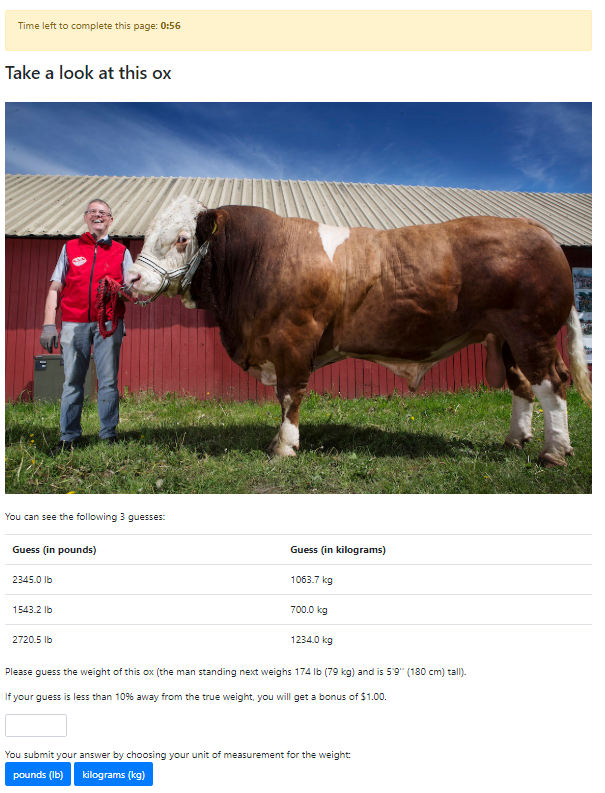
\includegraphics[width=.8\textwidth]{../Screenshots/FigS1.png}
\caption{Screendump of the choice-page in the dot-experiment with $d=403$ and $v=9$.}
\label{fig:S1}
\end{figure}

Our experimental setup on Mturk is simple. After accepting our ‘HIT’ (Mturk acronym for a ‘human intelligence task’) and providing informed consent, participants are asked to wait in a ‘waiting room’ until the ‘choice room’ becomes available. After entering the choice room, participants are asked to take a look at the image and make an estimate (see screenshot in Figure~\ref{fig:S1}). Depending on the view condition, participants can see $v\in\{0,1,3,9\}$ preceding estimates. We chose to present the ‘oldest’ previous estimate on the top of the list and the last estimate made on the bottom. When dealing with news, or financial data, users typically want to see the most recent activity first (think tweets, online banking transactions, news updates). With conversations it is different because there is a context to consider of whatever message came before and after the one you are looking at (think blogs or Facebook comments). We have chosen to use the conversation thread design (oldest on top) because there is no particular news criteria when guessing the weight of an ox or estimating the number of dots on a screen. Participants have one minute to think about the image and make their estimate. This might sound as a severe time constraint, but exploratory trials had shown that participants in general use less than a minute when performing this task. After submission, participants are thanked for their participation and the experiment ends. Waiting times are compensated with \$0.20 per minute (maximally 5 minutes), participation fee is \$0.10, and a bonus of \$1 is paid if an estimate is within 10\% of the true number.

\subsection*{Mturk settings and data quality}
When working with Mturk it is important to consider the right settings in order to obtain the best data quality possible \cite{chandler2016conducting}. Fair wage, attrition rates, removal of duplicate participants and informative feedback are some of the most important issues to address.

Average wage for participants in our experiments was $\sim$ \$12 per hour, which is considered good according to Mturk guidelines and certainly above the estimated average of \$6 per hour when excluding un-submitted and rejected work \cite{hara2018data}.

Quitting a study before completing it is prevalent on Mturk, and varies systemically across experimental conditions \cite{zhou2016pitfall}. On average 20 participants accepted our HITs within the first minute; after 10 minutes the average acceptance rate had dropped to 2-3 participants per minute and after an hour to less than one participant per minute. Our scripts were coded in such a way that participants were automatically assigned to a ‘waiting room’ in which they were asked to wait for maximally five minutes before entering the choice room. This meant that a lot of participants waited in vain. Due to such a high attrition rate in the first couple of experiments we changed the script slightly later on: Now the waiting room could contain a maximum of five participants, and when the waiting room was full, participants were told to come back and finish the HIT at a later point in time. This reduced the attrition rate to 6.5\% on average.

All participants automatically received an image-specific qualification when accepting a HIT. This qualification ensured that participants could not accept any other HITs that use the same image. Further data inspection showed that 32 participants somehow managed to accept two HITs with the same image anyway. The reason may be that the time interval between accepting two HITs with the same image was too short for the qualification to register in the Mturk interface. All 32 duplicate participants were removed before data analysis. In addition, we set the qualification that participants should have completed at least 100 HITs and have an accepted HIT rate of 98\% or above. This ensured that we would get only experienced and qualified participants.

Mturk participant attention was expected to be equal to or better than undergraduate participant’s attention \cite{hauser2016attentive}, while various forms of dishonesty (practical joking or telling others about the true value offline or on an Mturk participants web page) was expected to be rare. Our screening of data files before data analyses revealed that a small fraction of participants submitted ridiculously high estimates across images seen, thereby skewing thread averages substantially. These estimates were included in the calculations of the geometric mean of the social information. However, they were given a low weight determined from density estimates based on the control threads with $v=0$ (see section Modeled values above).

During our experiments, participants had easy access to our email for questions and possible bug reports. Apart from some minor difficulties when typing from a mobile device (less than 1\%) participants had few comments or complaints.

%\subsection*{Code and Software}
%All experiments are coded in the experimental software otree 2.1 \cite{chen2016otree} which is based on python and django. The code itself is designed along the same lines as the classical information cascade experiments by Anderson and Holt \cite{anderson1997information}. The main feature of any cascade game is that decisions are taken sequentially. A player makes an estimate, and the next one receives the information about the estimate of the previous player (or all or some previous players). Thus, the main technical issue is that only one person at a time can make a decision while others wait. As soon as a player finishes and leaves the choice page, the next player enters while all subsequent players still have to wait. Scripts for the analysis of data and for the plotting of all figures in the main text as well as in the Supplementary Information are available on \href{https://github.com/gavstrik/WoT}{github}.

%\subsection*{Data Collection}
%\label{dc}
%We obtained a total of 11748 estimates from 6196 unique participants. Any dot-image was only seen once by a participant, i.e. we had a total of 3157 participants seeing only one image, 1259 participants seeing two images, 1047 participants seeing three images, and 733 participants seeing all four images (either in the unmanipulated or manipulated conditions and with $v\in\{0,1,3,9\}$). A few of the manipulated threads were stopped prematurely (containing less than 100 participants) because early outlier estimates turned the social information available to the succeeding participants into unbelievably high numbers. In those threads, the transition period from compromizing to not at all believing the social information became very short, making the thread dynamics relative uninteresting. Instead of running a highly manipulated thread for a long time, we opted for restarting the thread with new participants. See Table~\ref{table:S1} for a full list of threads and their summary statistics.

%\subsection*{Outliers}
%Previous work has shown that distributions of independent estimates are approximately log-normal. Consequently, the arithmetic mean is usually much larger than most estimates and often larger than the true value. Testing our data we find distributions to be only approximately log-normal (see QQ-plots in Figure~\ref{fig: qq plots median}). In addition, Table~\ref{table:S1} shows highly variable distributions of estimates. Skewnesses and kurtoses, describing the lack of symmetry and the size of the tail of the distributions, span values from close to zero to above 100. These asymmetries are reflected by the presence of outliers.
%
%We did not remove any outlier, because the aggregate analysis and linear regression of thread medians is unaffected by the presence of outliers, except for possible larger confidence intervals. We
%%For all reported aggregate measures, outliers are removed if they have an error rate above 10, so that $|x_r-truth|/truth <10$, where $x_r$ is the estimate by participant $r$. We also use a lower bound of $truth/10$, due some reports of not being able to see the form input on mobile devices or unanticipated timeouts (see SI Appendix, section “Mturk Settings”). With these trimming criteria in place, we count a the following number of outliers: In the dots-experiments, 62 participants have an error rate above 100, and 118 participants have an error rate above 10, while 33 participants have made an estimate below 10\% of the true value. In the ox-experiments, one participant has an error rate above 30 and 9 participants have an error rate above 10, while 94 participants have made an estimate less than 10\% of the true value. This give a total of 151 (1.8 \%) outliers in the dots-experiments and 103 (4.1 \%) outliers in the ox-experiments, giving a grand total of 254 (2.4 \%) outliers out of 10.808 estimates.



%
%\section*{Supplementary data analysis}
%\subsection*{Summary Statistics}
%Figure~\ref{fig:sum_stats} shows the summary statistics of all historical (left) and manipulated (rigth) threads. As can be seen, as soon as participants can see preceding estimates, accuracy improves substantially in difficult tasks. Increasing the view count $v$ does not significantly improve collective accuracy in images with 55 and 148 dots. But as soon as the number of dots increases, social information starts to improve thread accuracy. And the larger the view count $v$, the more accurate the median (circles) becomes. Arithmetic means (triangles) quickly tend to overestimate the true value because free response elicitation of absolute values creates right-skewed, approximately log-normal distributions with a long tail, which inflate the means. Due to the outliers, means become highly uninformative. Galton disliked the use of the mean for this very reason as it “would give a voting power to ‘cranks’ in proportion to their crankiness” \cite{galton1907vox}. The interquartile and interdecile ranges show how high difficulty, $d$, leads to higher diversity (i.e. variation) in the dots-experiments, while a higher view-count tends to reduce variation when $d$ is fixed, although not always.
%
%The right hand side of Figure~\ref{fig:sum_stats} shows the equivalent results for manipulated threads. While participants are relatively unaffected by social information when difficulty is low in the unmanipulated threads, participants in the manipulated threads quick start to overestimate, even with $v=1$. For higher $d$'s and $v$'s, estimates inflate ever more. Clearly, in the begining of a thread, only a few of the observed estimates are high numbers, making it not so probable for new participants to get influenced by them. But when threads become longer, still more of the observed estimates are very high numbers, making it more difficult to resist their influence. At a certain point, all visible estimates may be so improbably high, that participants may suspect foul play and start to ignore them. In some threads this effect can be observed by estimates branching off into two directions: those estimates showing herd behaviour by following the extremely high estimates seen, and those estimates ignoring them. This may contribute to the high variance of the manipulated threads. Also note that for $v=1$, the medians of the manipulated threads are often much closer to the true value than it is the case in the corresponding controls. This is so because the size of the manipulation (in this case showing only the single highest estimate in the thread) is just about enough to compensate for the naturally occuring underestimations in the controls.


%
%\subsection*{Comparison across treatments}
%As mentioned in the main text, participants were allowed to participate in more than one of the treatments, but no participant was allowed to see the same image twice. We therefore have a substantial amount of participants who have seen either 2, 3 or 4 images. This makes it possible to compare individual persuadability scores across treatments. In Figure~\ref{compare} we have done so. The top plot shows the $\beta^w$-ordered result of comparisons across historical threads and the bottom plot shows the same for the manipulated threads. While the dot cloud in both plots is quite wide, there is a clear difference in the magnitude of persuadabilities and in the proportions of skeptics, compromisers, and persuadables. For the historical threads we can see, that almost all participants lie in the range between $0 < \beta^w < 0.5$, meaning that they keep their egocentric bias in line with \cite{rader2017advice}, but at the same time are highly flexible in their use of the social information provided. For the manipulated threads, we see a higher frequency of red colors and of $\beta^w$-values below zero, indicating that many participants did not agree with the social infomation they saw.


%references for the supp

\begin{thebibliography}{10}\scriptsize
\expandafter\ifx\csname url\endcsname\relax
  \def\url#1{\texttt{#1}}\fi
\expandafter\ifx\csname urlprefix\endcsname\relax\def\urlprefix{URL }\fi
\providecommand{\bibinfo}[2]{#2}
\providecommand{\eprint}[2][]{\url{#2}}


\bibitem{berinsky2012evaluating}
\bibinfo{author}{Berinsky, A.~J.}, \bibinfo{author}{Huber, G.~A.} \&
  \bibinfo{author}{Lenz, G.~S.}
\newblock \bibinfo{title}{Evaluating online labor markets for experimental
  research: Amazon. com's mechanical turk}.
\newblock \emph{\bibinfo{journal}{Polit Anal}} \textbf{\bibinfo{volume}{20}},
  \bibinfo{pages}{351--368} (\bibinfo{year}{2012}).

\bibitem{buhrmester2018evaluation}
\bibinfo{author}{Buhrmester, M.~D.}, \bibinfo{author}{Talaifar, S.} \&
  \bibinfo{author}{Gosling, S.~D.}
\newblock \bibinfo{title}{An evaluation of amazon’s mechanical turk, its
  rapid rise, and its effective use}.
\newblock \emph{\bibinfo{journal}{Perspect Psychol Sci}}
  \textbf{\bibinfo{volume}{13}}, \bibinfo{pages}{149--154}
  (\bibinfo{year}{2018}).

\bibitem{mason2009financial}
\bibinfo{author}{Mason, W.} \& \bibinfo{author}{Watts, D.~J.}
\newblock \bibinfo{title}{Financial incentives and the performance of crowds}.
\newblock In \emph{\bibinfo{booktitle}{Proceedings of the ACM SIGKDD workshop
  on human computation}}, \bibinfo{pages}{77--85} (\bibinfo{organization}{ACM},
  \bibinfo{year}{2009}).

\bibitem{buhrmester2011amazon}
\bibinfo{author}{Buhrmester, M.}, \bibinfo{author}{Kwang, T.} \&
  \bibinfo{author}{Gosling, S.~D.}
\newblock \bibinfo{title}{Amazon's mechanical turk: A new source of
  inexpensive, yet high-quality, data?}
\newblock \emph{\bibinfo{journal}{Perspect Psychol Sci}}
  \textbf{\bibinfo{volume}{6}}, \bibinfo{pages}{3--5} (\bibinfo{year}{2011}).

\bibitem{crump2013evaluating}
\bibinfo{author}{Crump, M.~J.}, \bibinfo{author}{McDonnell, J.~V.} \&
  \bibinfo{author}{Gureckis, T.~M.}
\newblock \bibinfo{title}{Evaluating amazon's mechanical turk as a tool for
  experimental behavioral research}.
\newblock \emph{\bibinfo{journal}{PLoS One}} \textbf{\bibinfo{volume}{8}},
  \bibinfo{pages}{e57410} (\bibinfo{year}{2013}).

\bibitem{rand2012promise}
\bibinfo{author}{Rand, D.~G.}
\newblock \bibinfo{title}{The promise of mechanical turk: How online labor
  markets can help theorists run behavioral experiments}.
\newblock \emph{\bibinfo{journal}{J Theor Biol}}
  \textbf{\bibinfo{volume}{299}}, \bibinfo{pages}{172--179}
  (\bibinfo{year}{2012}).

\bibitem{horton2011online}
\bibinfo{author}{Horton, J.~J.}, \bibinfo{author}{Rand, D.~G.} \&
  \bibinfo{author}{Zeckhauser, R.~J.}
\newblock \bibinfo{title}{The online laboratory: Conducting experiments in a
  real labor market}.
\newblock \emph{\bibinfo{journal}{Exper Econ}} \textbf{\bibinfo{volume}{14}},
  \bibinfo{pages}{399--425} (\bibinfo{year}{2011}).

\bibitem{chandler2016conducting}
\bibinfo{author}{Chandler, J.} \& \bibinfo{author}{Shapiro, D.}
\newblock \bibinfo{title}{Conducting clinical research using crowdsourced
  convenience samples}.
\newblock \emph{\bibinfo{journal}{Annu Rev Clin Psycho}}
  \textbf{\bibinfo{volume}{12}}, \bibinfo{pages}{53--81}
  (\bibinfo{year}{2016}).

\bibitem{hara2018data}
\bibinfo{author}{Hara, K.} \emph{et~al.}
\newblock \bibinfo{title}{A data-driven analysis of workers' earnings on amazon
  mechanical turk}.
\newblock In \emph{\bibinfo{booktitle}{Proceedings of the 2018 CHI Conference
  on Human Factors in Computing Systems}}, \bibinfo{pages}{449}
  (\bibinfo{organization}{ACM}, \bibinfo{year}{2018}).

\bibitem{zhou2016pitfall}
\bibinfo{author}{Zhou, H.} \& \bibinfo{author}{Fishbach, A.}
\newblock \bibinfo{title}{The pitfall of experimenting on the web: How
  unattended selective attrition leads to surprising (yet false) research
  conclusions.}
\newblock \emph{\bibinfo{journal}{J Pers Soc Psychol}}
  \textbf{\bibinfo{volume}{111}}, \bibinfo{pages}{493} (\bibinfo{year}{2016}).

\bibitem{hauser2016attentive}
\bibinfo{author}{Hauser, D.~J.} \& \bibinfo{author}{Schwarz, N.}
\newblock \bibinfo{title}{Attentive turkers: Mturk participants perform better
  on online attention checks than do subject pool participants}.
\newblock \emph{\bibinfo{journal}{Behavior research methods}}
  \textbf{\bibinfo{volume}{48}}, \bibinfo{pages}{400--407}
  (\bibinfo{year}{2016}).
 
 \end{thebibliography}
  


\newpage

\begin{figure}%[!h]
	\centering
	\hspace{-20px}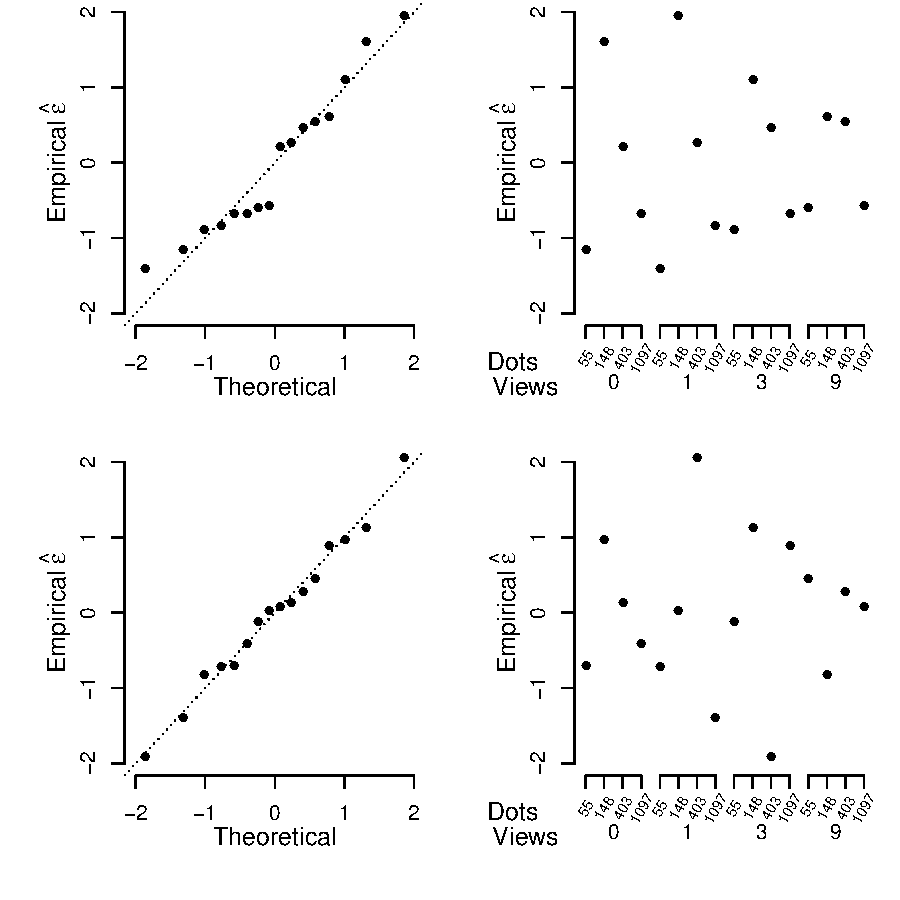
\includegraphics[width=.75\textwidth]{qqplots_median.pdf}
	\caption{Model diagnostic plots for median analysis. Top left: QQ plot for the residuals from the historical thread medians analysis. Top right: the same residuals plottet against session groups. Bottom left: QQ plot for the residuals from the manipulated thread medians analysis. Bottom right: the same residuals plottet against session groups.}
	\label{fig: qq plots median}
\end{figure}
\newpage

\begin{figure}%[!h]
\centering
	\hspace{-30px}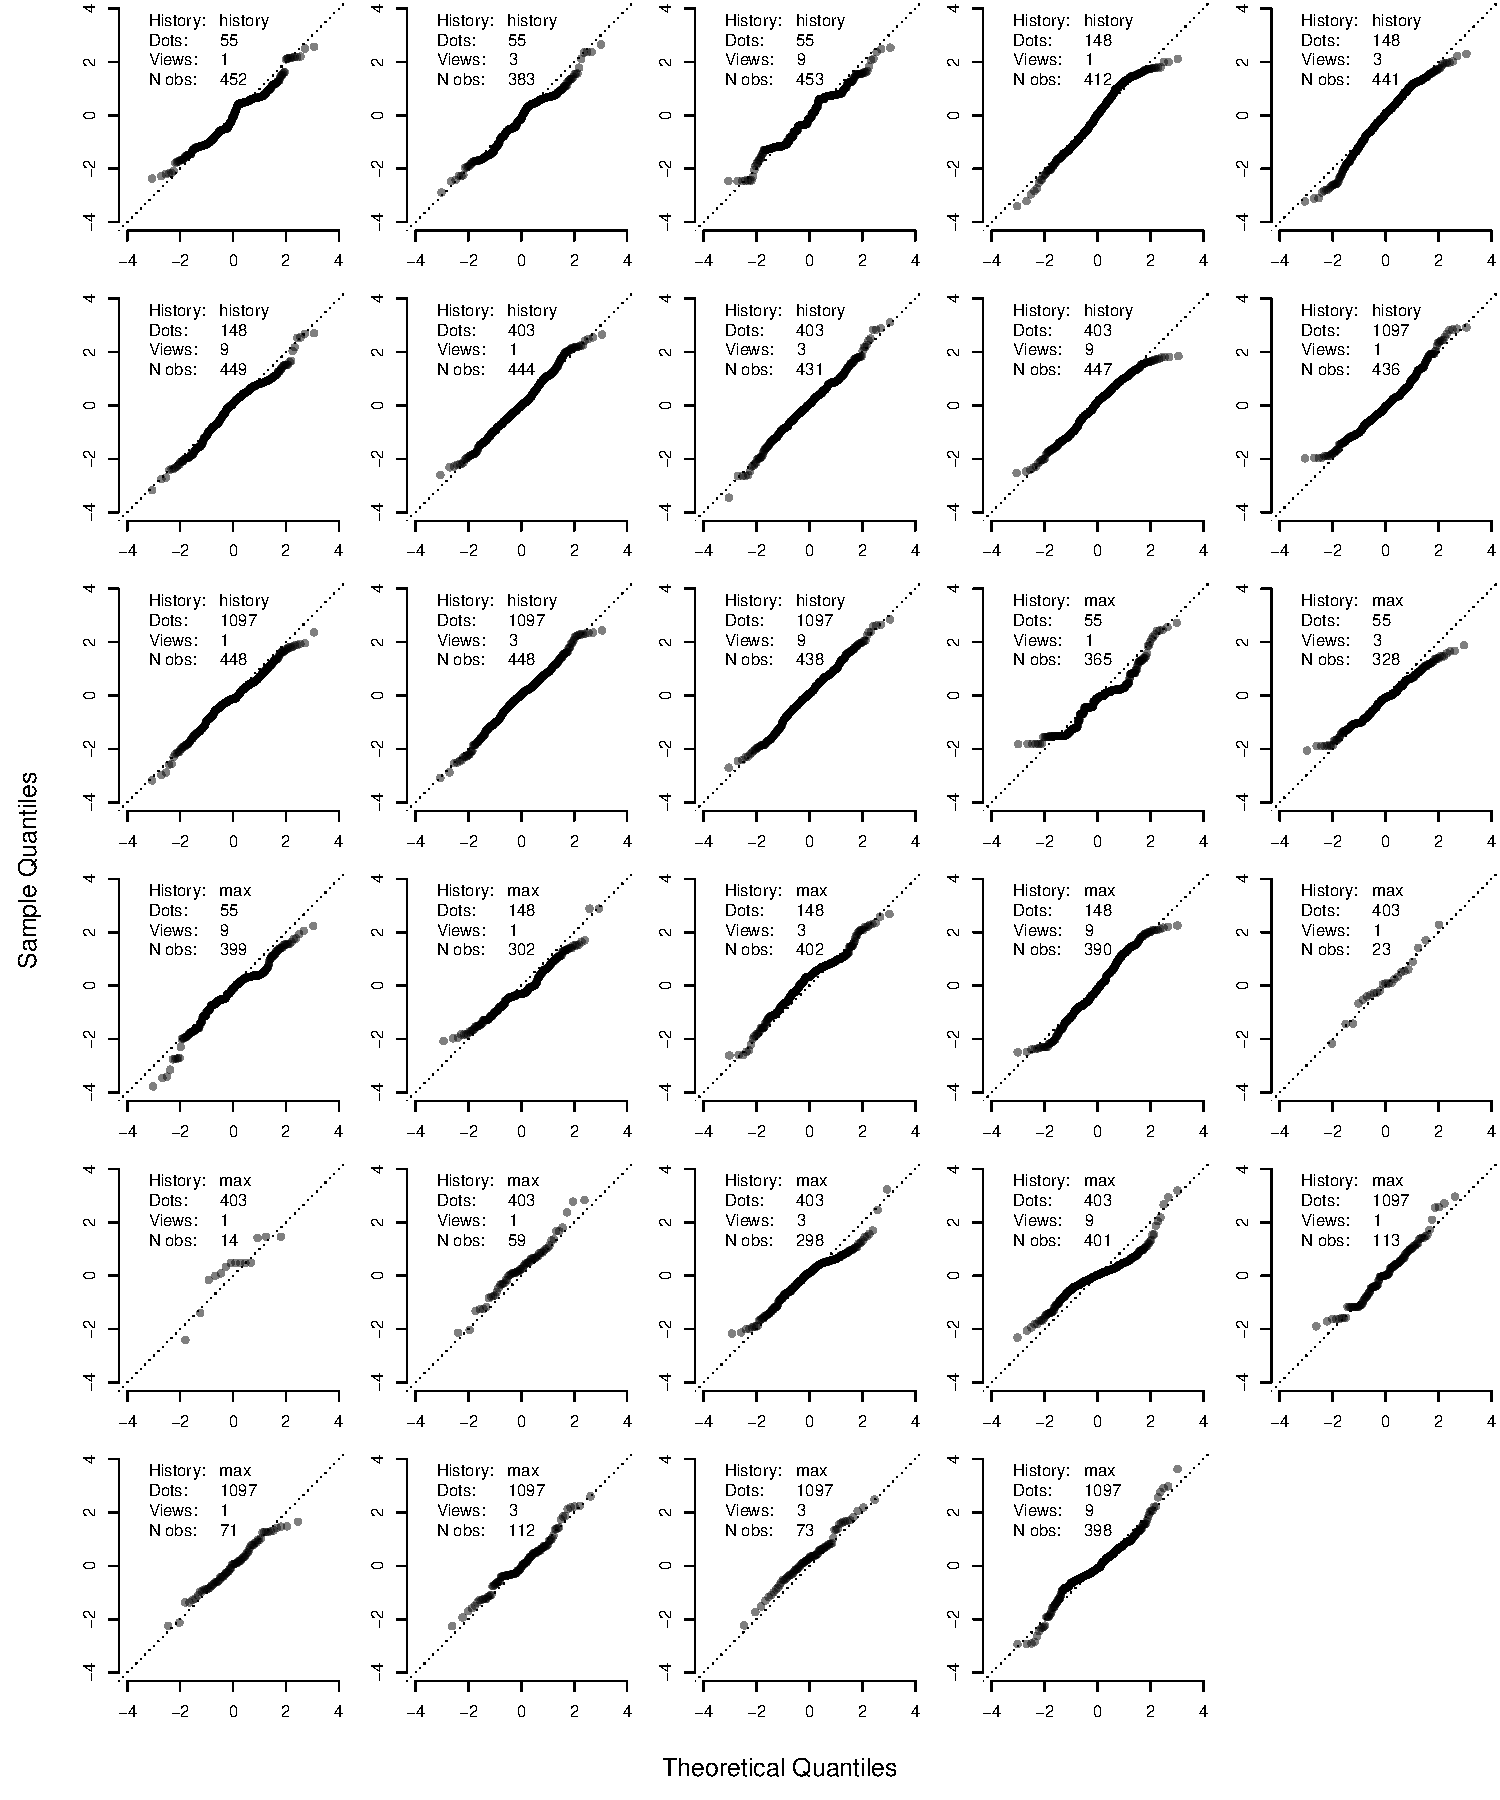
\includegraphics[width=1\linewidth]{qqplots}
	\caption{QQ-plots for the 29 unique threads from Amazon Mechanical Turk experiments. With some exceptions, the models fit fairly well. Some series with very few observations are discarded in the analysis.}\label{fig: QQ plots AMT}
\end{figure}
\newpage

\begin{figure}%[!h]
\centering
	\hspace{-30px}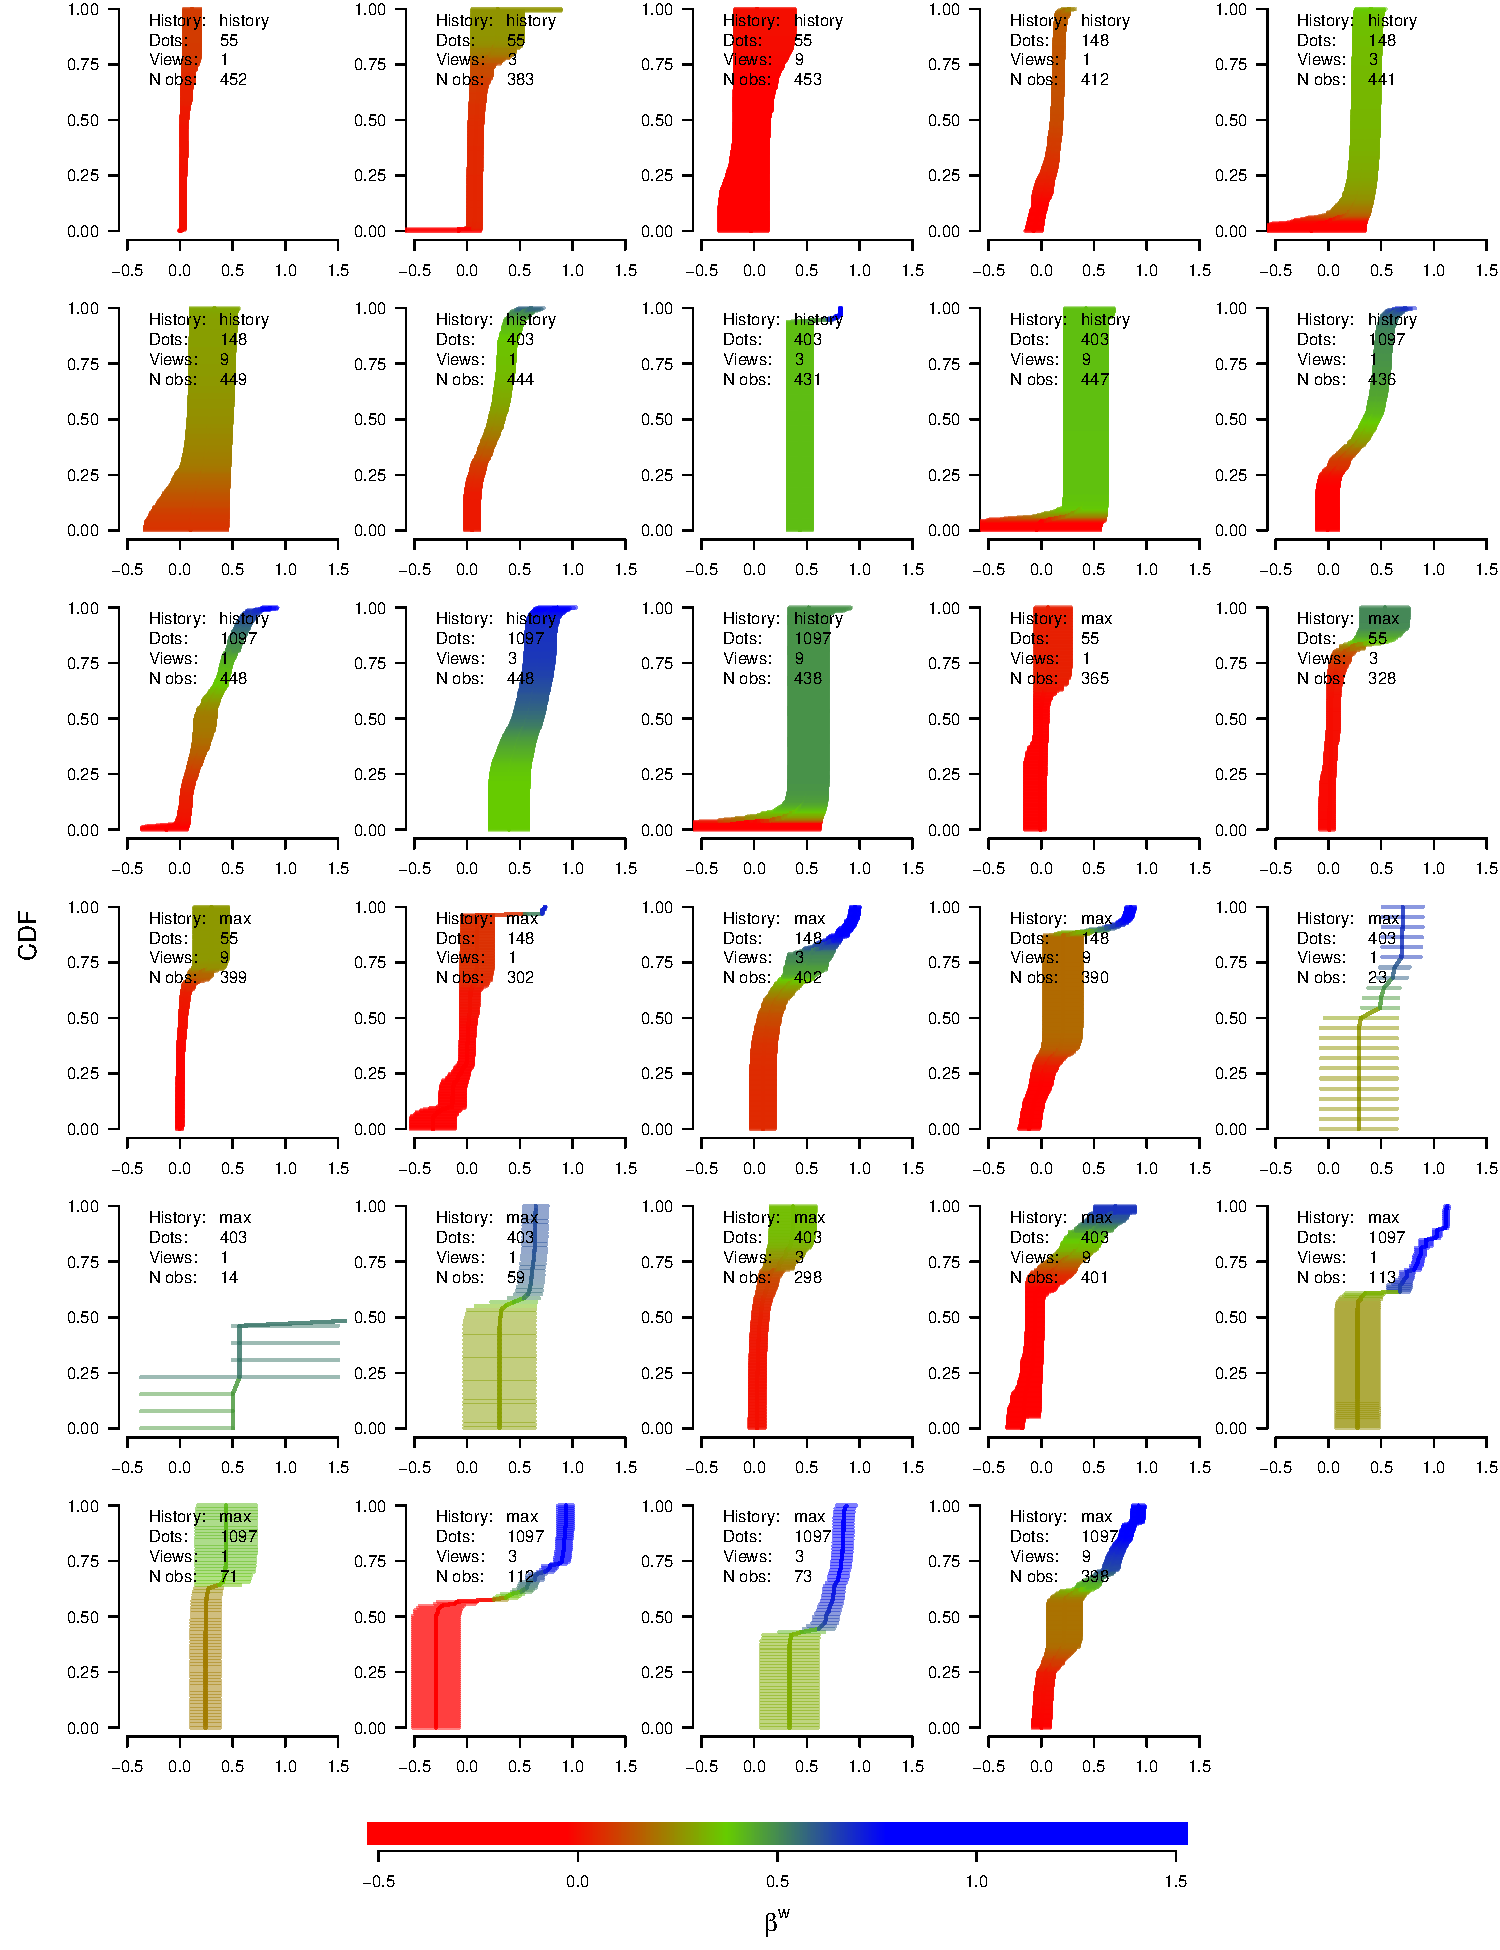
\includegraphics[width=1\linewidth]{allbetas}
	\caption{Distributions of estimated $\beta^w$'s for each thread. Color scale is fixed across all threads. Red colors indicate skeptics, blue colors indicate persuadables and green colors indicate compromisers.}\label{fig: weighted beta distributions}
\end{figure}
\newpage

\begin{figure}%[!h]
\centering
	\hspace{-30px}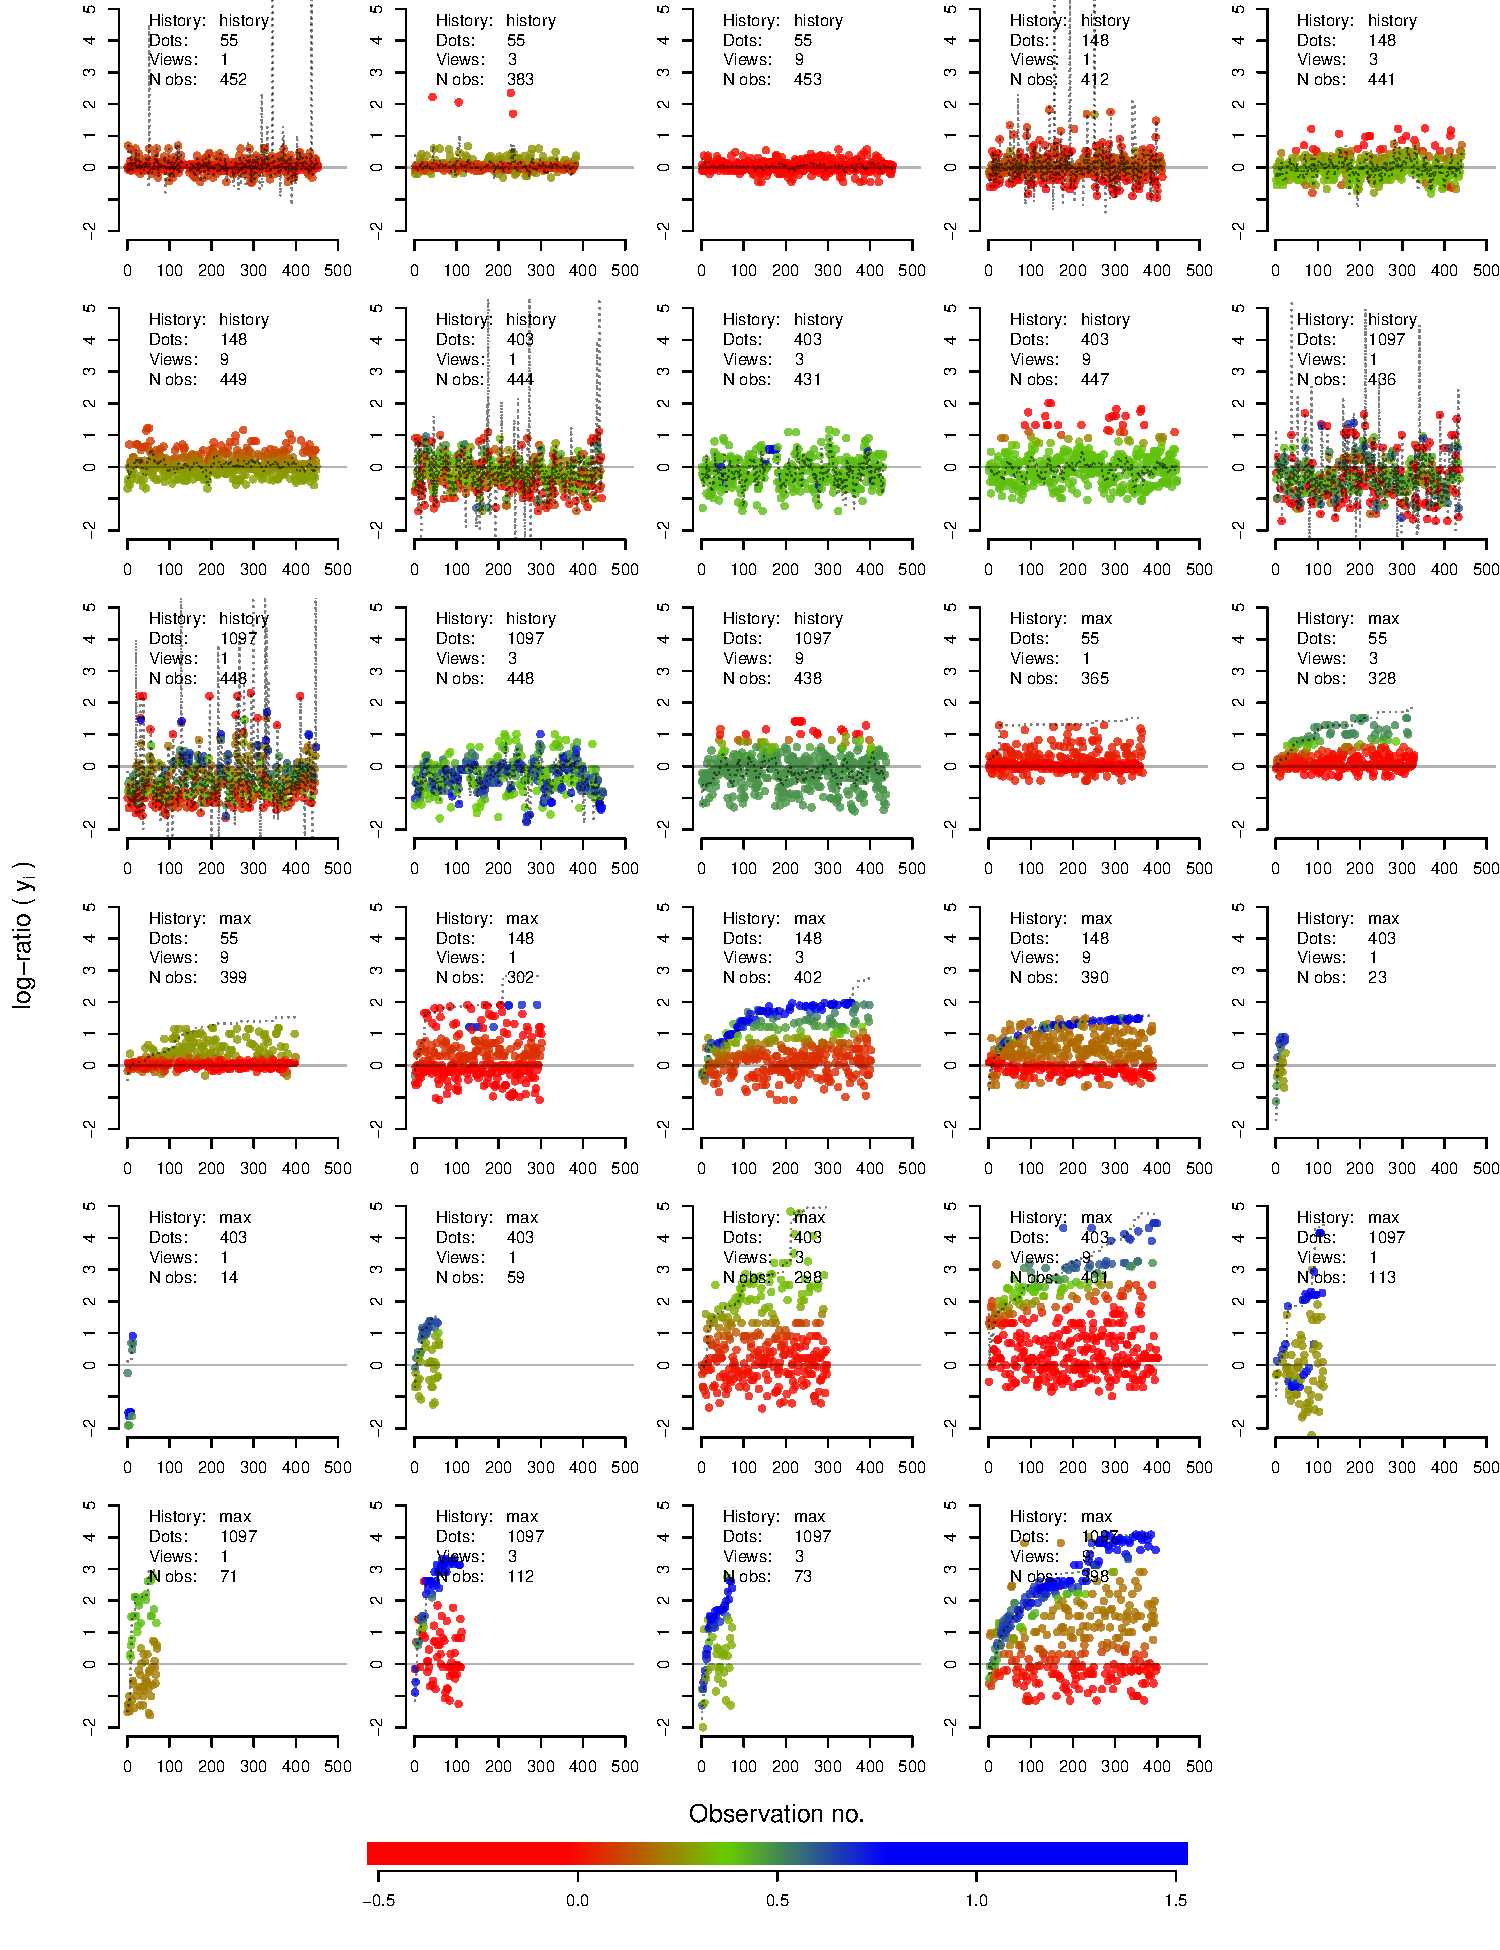
\includegraphics[width=1\linewidth]{allthreads}
	\caption{Individual guesses for each thread, colored by their estimated $\beta^w$ values. Social information available at each timepoint is shown as dashed black lines. The $\beta^w$ color scale is fixed across all threads. Red colors indicate skeptics, blue colors indicate persuadables and green colors indicate compromisers.}\label{fig: threads with social info and colored by beta weights}
\end{figure}
\newpage

\begin{figure}%[!h]
\centering
	\hspace{-30px}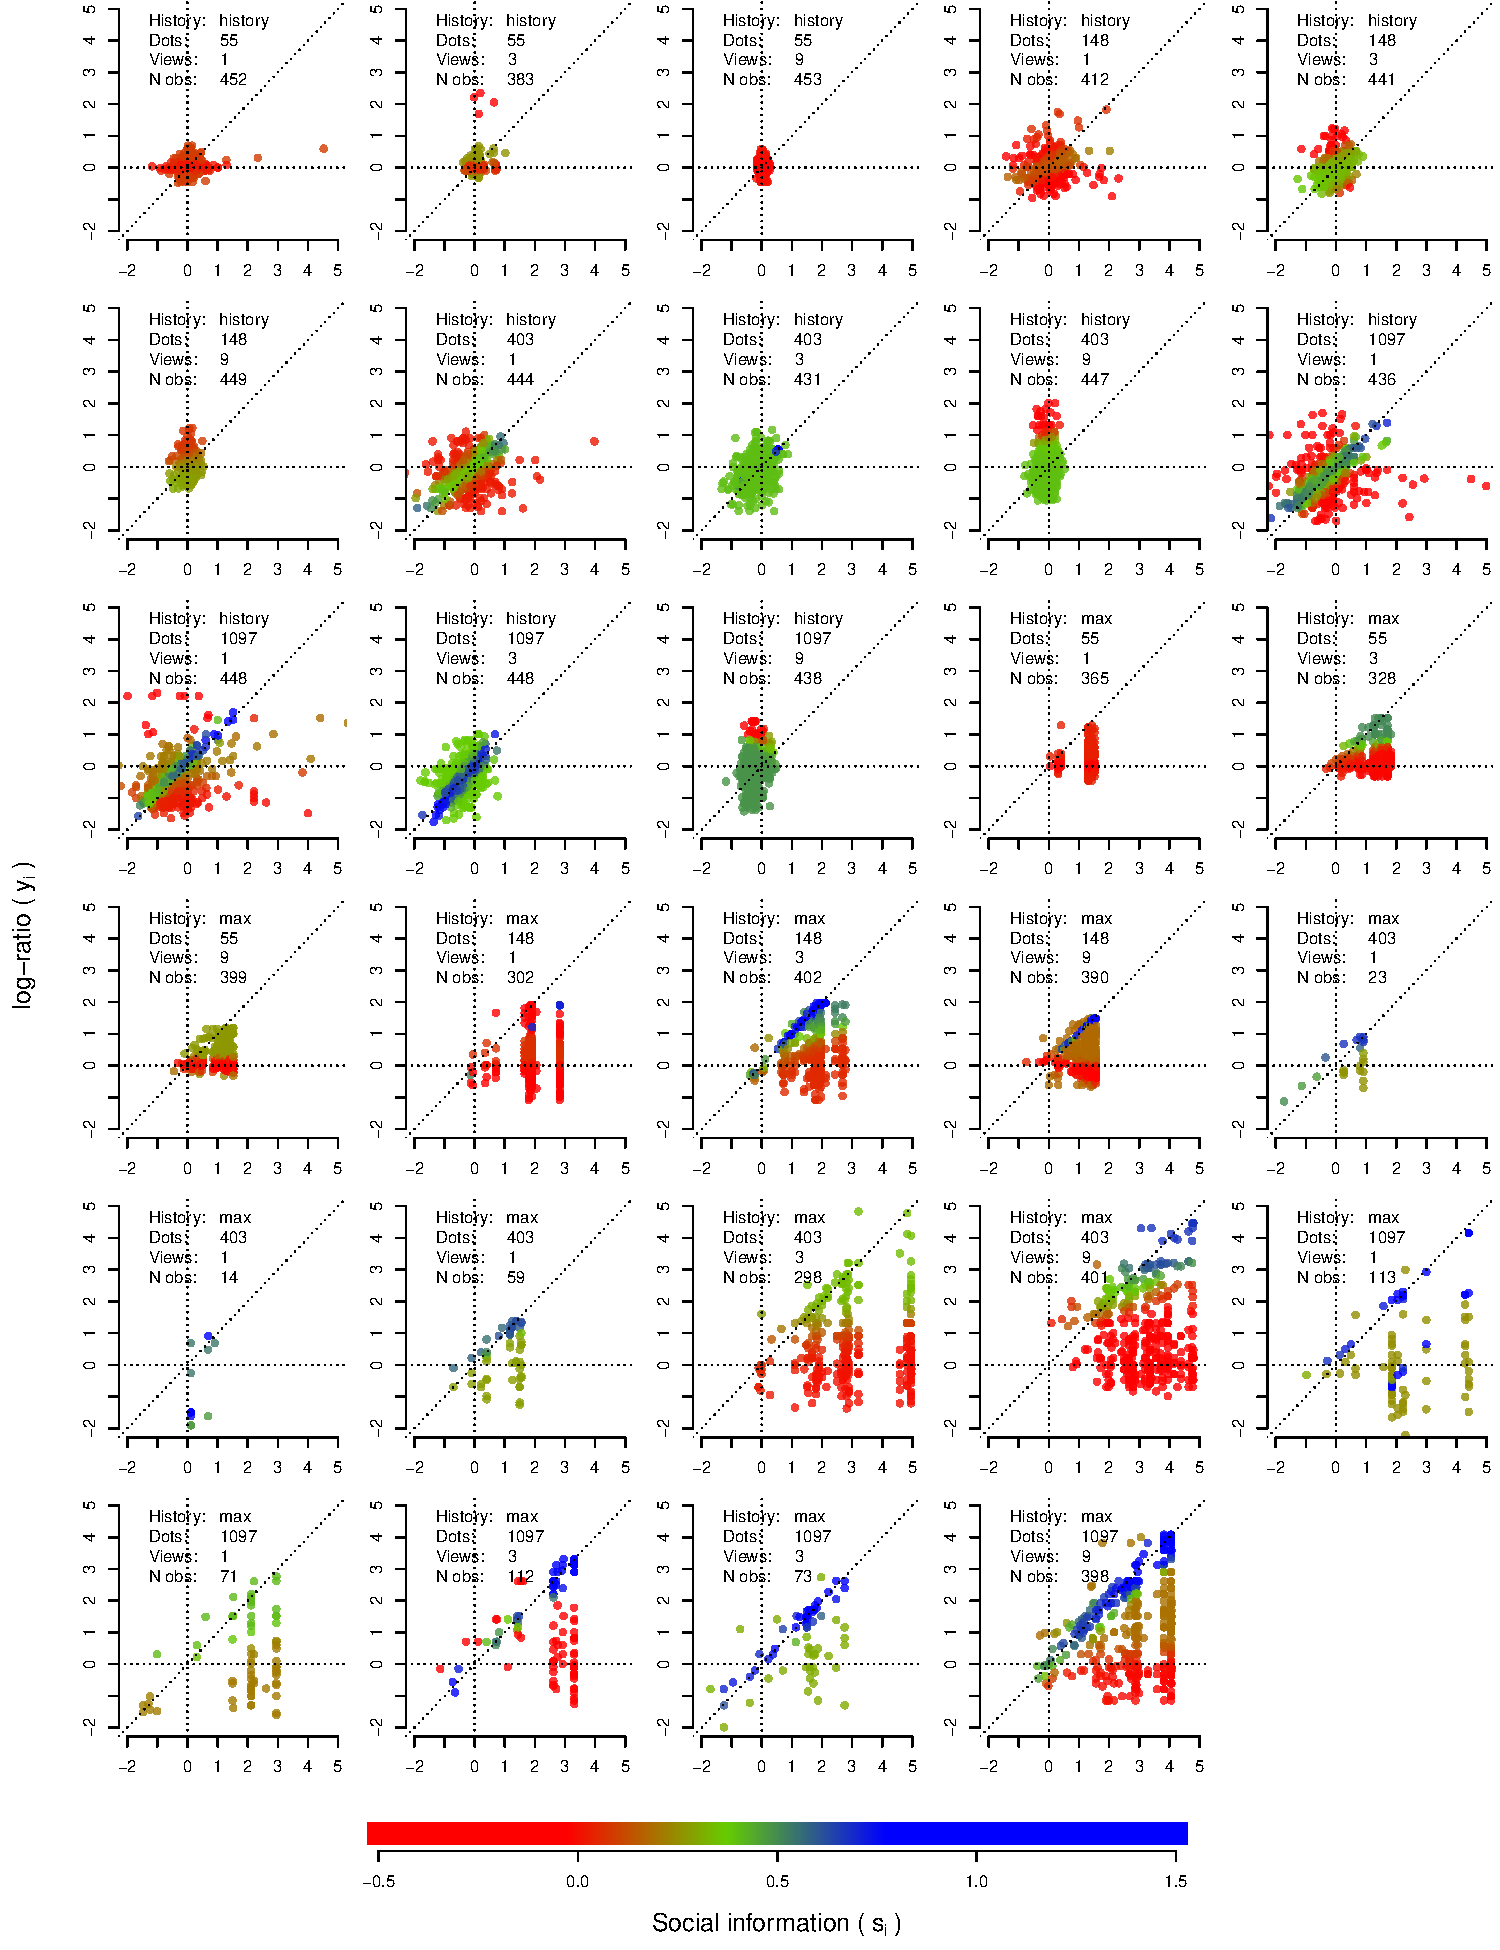
\includegraphics[width=1\linewidth]{allinfo}
	\caption{Actual estimates by each participant against the given social information. Colored by the estimated $\beta^w$ values. Color scale is fixed across all threads. Red colors indicate skeptics, blue colors indicate persuadables and green colors indicate compromisers.}\label{fig: social info vs estimates}
\end{figure}
\newpage

\begin{table}\centering
\caption{\textbf{Data Table of threads:}  method: type of thread - `history' are pristine threads where participants see the $v$ preceding estimates and `max' are manipulated threads where participants see the $v$ highest estimates made so far in the thread; $d$: number of dots in image; $v$ = number of visible previous estimates; $N$ = thread length; median = median of thread; mean = mean of thread; SD = standard deviation; CV = coefficient of variation; skew = skewness; kurt = kurtosis; bonus = percentage of estimates within 10 \% of the true value.}

\begin{tabular}{lrrlrrrrrrrr}
\hline
 method   &    $d$ &   $v$ & thread id  &   $N$ &   median &     mean &       SD &    CV &   skew &   kurt &   bonus (\%) \\
\hline
 history  &   55 &   0 & fscmakcz & 464 &     55   &  2360.57 & 42038.6  & 17.81 &  21.01 & 445.08 &        60.99 \\
 history  &   55 &   1 & hs6bovtz & 477 &     57   &  1682.13 & 29381.7  & 17.47 &  21.18 & 453.74 &        57.02 \\
 history  &   55 &   3 & 3cda8qpn & 405 &     56   &  8320.59 & 73524.4  &  8.84 &   9.59 &  93.58 &        66.91 \\
 history  &   55 &   9 & bvpj37io & 476 &     56   &  1239.85 & 25435.5  & 20.51 &  21.74 & 470.87 &        56.09 \\
 history  &  148 &   0 & dwnjf9mb & 464 &    140   &  1349.14 & 12891    &  9.55 &  12.83 & 172.18 &        22.41 \\
 history  &  148 &   1 & ehaxc7lu & 435 &    150   &  2250.86 & 27802.5  & 12.35 &  15.66 & 261.32 &        25.75 \\
 history  &  148 &   3 & ck291lk5 & 466 &    147.5 &  2523.51 & 38071.3  & 15.09 &  20.42 & 427.38 &        23.18 \\
 history  &  148 &   9 & 2hxe3g0w & 473 &    153   &  3182.51 & 38085.7  & 11.97 &  13.85 & 196.79 &        24.52 \\
 history  &  403 &   0 & hqx0v7t5 & 473 &    300   &  4816.02 & 49624.9  & 10.3  &  14.16 & 220.03 &         7.82 \\
 history  &  403 &   1 & 9bbkjlye & 469 &    320   &  2791.59 & 31667.6  & 11.34 &  15.23 & 248.43 &         8.1  \\
 history  &  403 &   3 & 5du4txa7 & 455 &    350   &  2430    & 29944.3  & 12.32 &  15.25 & 233.19 &        11.65 \\
 history  &  403 &   9 & spw8qdcd & 470 &    400   &  3035.65 & 36078.8  & 11.89 &  15.32 & 235.27 &        10.43 \\
 history  & 1097 &   0 & hal5jdl0 & 423 &    657   &  8855.13 & 76379.1  &  8.63 &  11.46 & 138.21 &         9.69 \\
 history  & 1097 &   1 & huyygtho & 461 &    750   &  2924.95 & 25012.2  &  8.55 &  17.91 & 344.84 &         9.76 \\
 history  & 1097 &   1 & z0rvh02v & 473 &    650   &  8091.24 & 68728.9  &  8.49 &  11.74 & 144.62 &         8.67 \\
 history  & 1097 &   3 & hhb0if6e & 470 &    812.5 &  4811.97 & 53329.9  & 11.08 &  15.61 & 259.91 &        20.64 \\
 history  & 1097 &   9 & wv4xujg7 & 460 &    999   &  2748    & 31206.8  & 11.36 &  21.24 & 451.09 &        13.7  \\
 max      &   55 &   1 & aebicytb & 384 &     57   &    68.7  &    35.77 &  0.52 &   2.82 &   8.76 &        54.17 \\
 max      &   55 &   3 & 094p61xp & 340 &     60   &   101.05 &   413.25 &  4.09 &  18    & 326.23 &        43.82 \\
 max      &   55 &   9 & 8c80yyxl & 418 &     60   &    75.03 &    45.69 &  0.61 &   4.72 &  34.23 &        51.44 \\
 max      &  148 &   1 & 78wuly7l & 317 &    152   &   271.06 &   323.75 &  1.19 &   3.84 &  19.06 &        17.03 \\
 max      &  148 &   3 & u2sxnl2p & 418 &    220   &   366.6  &   596    &  1.63 &  11.6  & 179.79 &         9.57 \\
 max      &  148 &   9 & mf57hnwb & 412 &    210   &   266.74 &   168.39 &  0.63 &   1.08 &   0.2  &        12.38 \\
 max      &  403 &   1 & 1r17post &  25 &    400   &   549    &   402.64 &  0.73 &   1.83 &   4.14 &         4    \\
 max      &  403 &   1 & 6c4s02ki &  16 &     90   &   452.5  &   614.18 &  1.36 &   2.26 &   4.85 &         0    \\
 max      &  403 &   1 & e8vv9575 &  64 &    600   &   734.38 &   506.71 &  0.69 &   0.48 &  -1    &         6.25 \\
 max      &  403 &   3 & ua2230ux & 315 &    600   &  3215.08 &  9635.18 &  3    &   4.84 &  22.79 &         8.25 \\
 max      &  403 &   9 & 1xyev3dj & 422 &    887.5 &  4758.88 & 25397.5  &  5.34 &  17.68 & 339.78 &         8.29 \\
 max      & 1097 &   1 & 7yqp8bxc & 116 &    800   &  5463.93 & 15517.2  &  2.84 &   4.21 &  16.95 &         8.62 \\
 max      & 1097 &   1 & q5brhgnz &  76 &   1062.5 &  3310.3  &  4690.72 &  1.42 &   2.13 &   4.19 &         5.26 \\
 max      & 1097 &   3 & 2x6km84z & 117 &   2500   &  7593.38 &  9341.25 &  1.23 &   1.29 &   0.35 &        13.68 \\
 max      & 1097 &   3 & ud5vo371 &  78 &   2950   &  5167.06 & 12588.5  &  2.44 &   7.43 &  58.71 &         3.85 \\
 max      & 1097 &   9 & lh7wb36v & 416 &   3410   & 13024.2  & 38664.1  &  2.97 &  11.9  & 183.47 &         8.17 \\
\hline
 &&&& 11.748 &&&&&&&
\\
%\bottomrule
\end{tabular}
\end{table}\label{table:S1}



\end{document}
